\documentclass[letterpaper,11pt]{article}
\usepackage[parfill]{parskip} % Remove paragraph indentation
\usepackage{amsmath}
\usepackage{float}
\usepackage[margin=1in]{geometry}
\usepackage{graphicx}
\usepackage{placeins}
\usepackage{siunitx}
\usepackage[title]{appendix}
\usepackage{pdflscape}
\usepackage{tabularx}
\usepackage{times}
\usepackage{url}
\usepackage{setspace}
\usepackage[none]{hyphenat}
\usepackage{pdfpages}
\usepackage{longtable}
\usepackage{tikz}
\usepackage{hyperref}
\usepackage{minted}

\DeclareSIUnit{\samplepersec}{SPS}
\newcommand{\code}[1]{\mintinline{text}{#1}}

\begin{document}

\begin{titlepage}
    \begin{center}
        \vspace*{1cm}

        \Large
        \textbf{ELEC 490/498 Project Final Report}

        \vspace{0.5cm}
        Group 18\\
        TeachEE: Accessible Electronics Instrumentation\\
        \vspace{0.5cm}
        \normalsize
        \textbf{John Giorshev (20103586, john.giorshev@queensu.ca) \\ Eric Yang (20120750, e.yang@queensu.ca) \\ Ethan Peterson (20105011, 17emp5@queensu.ca) \\ Timothy Morland (20096286, 17tm22@queensu.ca)}\\
        \vspace{0.5cm}
        Submitted April 10, 2023\\

        \vfill
            
        \textbf{To:}\\
        Instructor Dr. Michael Korenberg (korenber@queensu.ca) \\
        Instructor Dr. Alireza Bakhshai (alireza.bakhshai@queensu.ca) \\
        Instructor Dr. Alex Tait (alex.tait@queensu.ca) \\
        Instructor and Supervisor Dr. Sean Whitehall (sw109@queensu.ca) \\
        Supervisor Dr. Thomas Dean (tom.dean@queensu.ca) \\
            
        \vspace{1.8cm}

    \end{center}
\end{titlepage}
\setstretch{1.5}
\pagenumbering{gobble}
\section*{Executive Summary}
% ERIC OWNS THIS SECTION
The Covid-19 pandemic abruptly forced educational institutions towards online
learning. As a result, many of these institutions were unequipped to deal with
this new learning model. Much of the onsite equipment, such as oscilloscopes and
signal generators, is ill-suited for online learning due to its high cost and
poor portability. Additionally, the take-home equipment provided to students
during the pandemic was typically of lower quality in comparison. In particular,
the oscilloscopes provided by the Electronics II course taught at Queen's
University were expensive and of poor quality. They had tiny 3-inch displays and
a small maximum bandwidth of 100 kHz. Moreover, they were single channel,
limiting the student's ability to see how signals in a circuit are related to
one another.

TeachEE is a general-purpose electronics measurement instrument designed for remote
engineering labs, functioning as both an oscilloscope and current monitor. It bundles
together the functionality most required in Electrical Engineering labs and packages
it with lightweight and portable software. 

TeachEE's hardware consists of a four-layer custom designed PCB powered by a USB
connection to the computer. The PCB has a two-channel 1MSPS ADC for reading low-speed
signals and current from a hall-effect sensor. The PCB also has a two-channel 40MSPS
ADC for observing high speed signals. Both ADCs are connected to an FPGA, which is in
turn connected to USB 2.0 PHY. The FPGA collects sample data from both ADCs and frames
it into packets, which are sent over the USB PHY and transmitted to the computer to be
decoded and displayed. This allows TeachEE to leverage the student's machine to create
a streamlined user experience. 

TeachEE's software is a full stack application written in Rust. Its workload is split
between three modules, each of which runs in its own thread. The first module is the
USB Manager, responsible for reading and decoding packets from the hardware driver
into voltage and current samples. The second is the App, responsible for updating and
displaying the user interface. The third module, the Controller, facilitates
communication between the two, and performs signal triggering and frequency spectrum
analysis. These three threads pass samples between each other using two sets of two
buffers: the USB Buffers and App Buffers. By cycling between buffers within a set,
much of the data processing can be parallelized, greatly improving performance. 

\newpage

\setstretch{1}
\tableofcontents
\listoffigures
\listoftables
\newpage
% upgraded this to double spacing as per report formatting reqs
\setstretch{2}
\pagenumbering{arabic}
\section{Motivation \& Background}
% ERIC
% Motivation and background – a clear problem statement and the motivation for the
% project (why is it technologically interesting?). A good motivation argument
% usually relies on facts and figures about the technological void that you seek
% to fill with your design. Back-up your facts and figures by referencing archival
% references. Examples of archival references include: journal papers, conference
% papers, patents, books, corporate technical and annual reports, application
% notes. Use the standard IEEE citation format. Website URLs are not archival
During the Covid-19 pandemic, universities abruptly switched to remote learning
as campuses were shut down. This sudden change exposed the lack of support for
digital learning models \cite{online_learning}. Although the pandemic has since
passed, forward-thinking institutions are starting to invest in online programs,
for example, by leveraging AI chatbots and teaching assistants. Additionally,
online course providers such as Udemy have recently risen in popularity as a
cheap alternative to traditional postsecondary education. With this trend of
remote higher education, engineering students will need their own lab equipment
to complete their learning requirements.

TeachEE is a general-purpose electronics measurement instrument
designed for remotely delivered engineering labs. It acts as both a
USB oscilloscope and current monitor. Currently, there are few instrumentation
options for students completing their labs remotely. The oscilloscopes used for
onsite learning are bulky and difficult to use. TeachEE bundles
together the functionality most commonly required for electrical engineering
labs and packages it with portable software that can run on lower end computers
with any operating system.

As TeachEE is targeted for electrical engineering students, it must be powerful
enough for use in a variety of practices, but also simple and intuitive enough
for novices. It must be compact, to be carried between classes, and
operating-system agnostic, to ensure that students can use it with any machine.
Finally, TeachEE must be cost-efficient, so that students can justify purchasing
this oscilloscope as opposed to alternatives.

\section{Design}
%% Design – describe your functional requirements and constraints; provide
%% technical details about your design process for meeting the project goals;
%% this might include identifying subsystems, analysis, modeling, and key
%% decisions made. If your project involves circuit design, you should describe
%% the simulations used to create your design

% Summarize Design process of hardware, fpga and SW. Make a brief note about how
% we parallelized much of the work by modelling the data as a byte stream.
% allowing for significant dev work without physical HW in house.

The TeachEE design is derived from the system requirements set in the blueprint
report. Given in Table \ref{tab:hw-reqs} and \ref{tab:sw-reqs} are the most important hardware
and software requirements respectively. It should also be noted that the FPGA
shares responsibility with the desktop application for fulfilling software
requirements.

\begin{table}[H]
    \caption{Hardware Requirements}
    \begin{tabularx}{\textwidth}{l|l|l|l}
          & Specification & Target Value & Tolerance \\
        \hline
        1 &Voltage Input Bandwidth&\SI{100}{\kilo\hertz}& $\pm \SI{1}{\kilo\hertz}$ \\
        2 &Current Input Bandwidth&\SI{100}{\kilo\hertz}& $\pm \SI{1}{\kilo\hertz}$ \\
        3 &Number of Current Input Channels& $1$ & $0$ \\ 
        4 &Number of Voltage Input Channels& $1$ & $+2$ \\
        5 &Voltage Sample Rate& \SI{1}{\mega\samplepersec} & \SI{0}{\mega\samplepersec}\\
        6 &Current Sample Rate& \SI{1}{\mega\samplepersec} & \SI{0}{\mega\samplepersec} \\
    \end{tabularx} 
\label{tab:hw-reqs}
\end{table}

\begin{table}[H]
  \caption{Software Requirements}
  \begin{tabularx}{\textwidth}{l|l}
    \textbf{1} & \textbf{Functional Requirements}\\
    \hline
    1.1 & The software shall be able to modify the horizontal and vertical scales of the plot. \\
    1.2 & The software shall be able to modify the trigger voltage. \\
    1.3 & The application shall be deployable to Windows, macOS, and Linux. \\
    \hline
    \textbf{2} & \textbf{Interface Requirements} \\
    \hline
    2.1 & The software shall be able to capture voltage samples and export them to a CSV file. \\
    2.2 & The software shall receive samples via the FTDI 232 in synchronous mode. \\
    \hline
    \textbf{3} & \textbf{Performance Requirements} \\
    \hline
    3.1 & The software shall be able to render waveforms at a rate of \SI{30}{\hertz} on screen.
  \end{tabularx} 
  \label{tab:sw-reqs}
\end{table}

Based on the system requirements, the project is divided into three
subsystems; hardware, FPGA, and software. The following subsections correspond
to each subsystem, each describing the subsystem's top level design and
key design decisions made to comply with system requirements.

% INCLUDE THE BLOCK DIAGRAMS FOR EACH OF THESE
% Talk about old design (from blueprint)
\subsection{Hardware} % Ethan
The primary design driving requirements for the Printed Circuit Board (PCB) are
the bandwidth and sample rate of the data acquisition channels. Bandwidth and
sample rate constrain the selection of the input filters and Analog to Digital
Converters (ADCs) on the PCB. After selecting these parts, they can be easily
duplicated to add additional channels. A full requirement
compliance check for the hardware and other subsystems is provided in Section
\ref{sec:testing}.

Given the requirement for a single voltage and current channel with room for
additional voltage channels, the team settled on a four-channel design. One ADC
channel would be used for current and another for voltage. The remaining two
channels would be made available to be implemented as a stretch goal. The two
spare channels would also have a higher sample rate to improve the utility of
the instrument.

The data acquisition channels are connected to an FPGA rather than a
microprocessor. This decision was made to prevent real time data processing
limitations and ensure precise timing in the sampling of the signal waveforms.
Moreover, an FPGA or ASIC is commonly used in existing commercial
oscilloscopes to fulfill these real time requirements. A compromise that was
made in the design was the use of an FPGA module, rather than installing
the chip to the PCB directly. While such a module could not be used in TeachEE
in a mass-production setting, it greatly shortened the PCB design time, and
allows the FPGA to be easily replaced in the event of hardware failure.
Additionally, the FPGA combines all the sample streams and provides a single
point of contact to the USB interface.

Figure \ref{fig:hw-block-diagram} is a complete hardware block diagram used as a
guide for the PCB design implementation.

\begin{figure}[H]
  \centering
  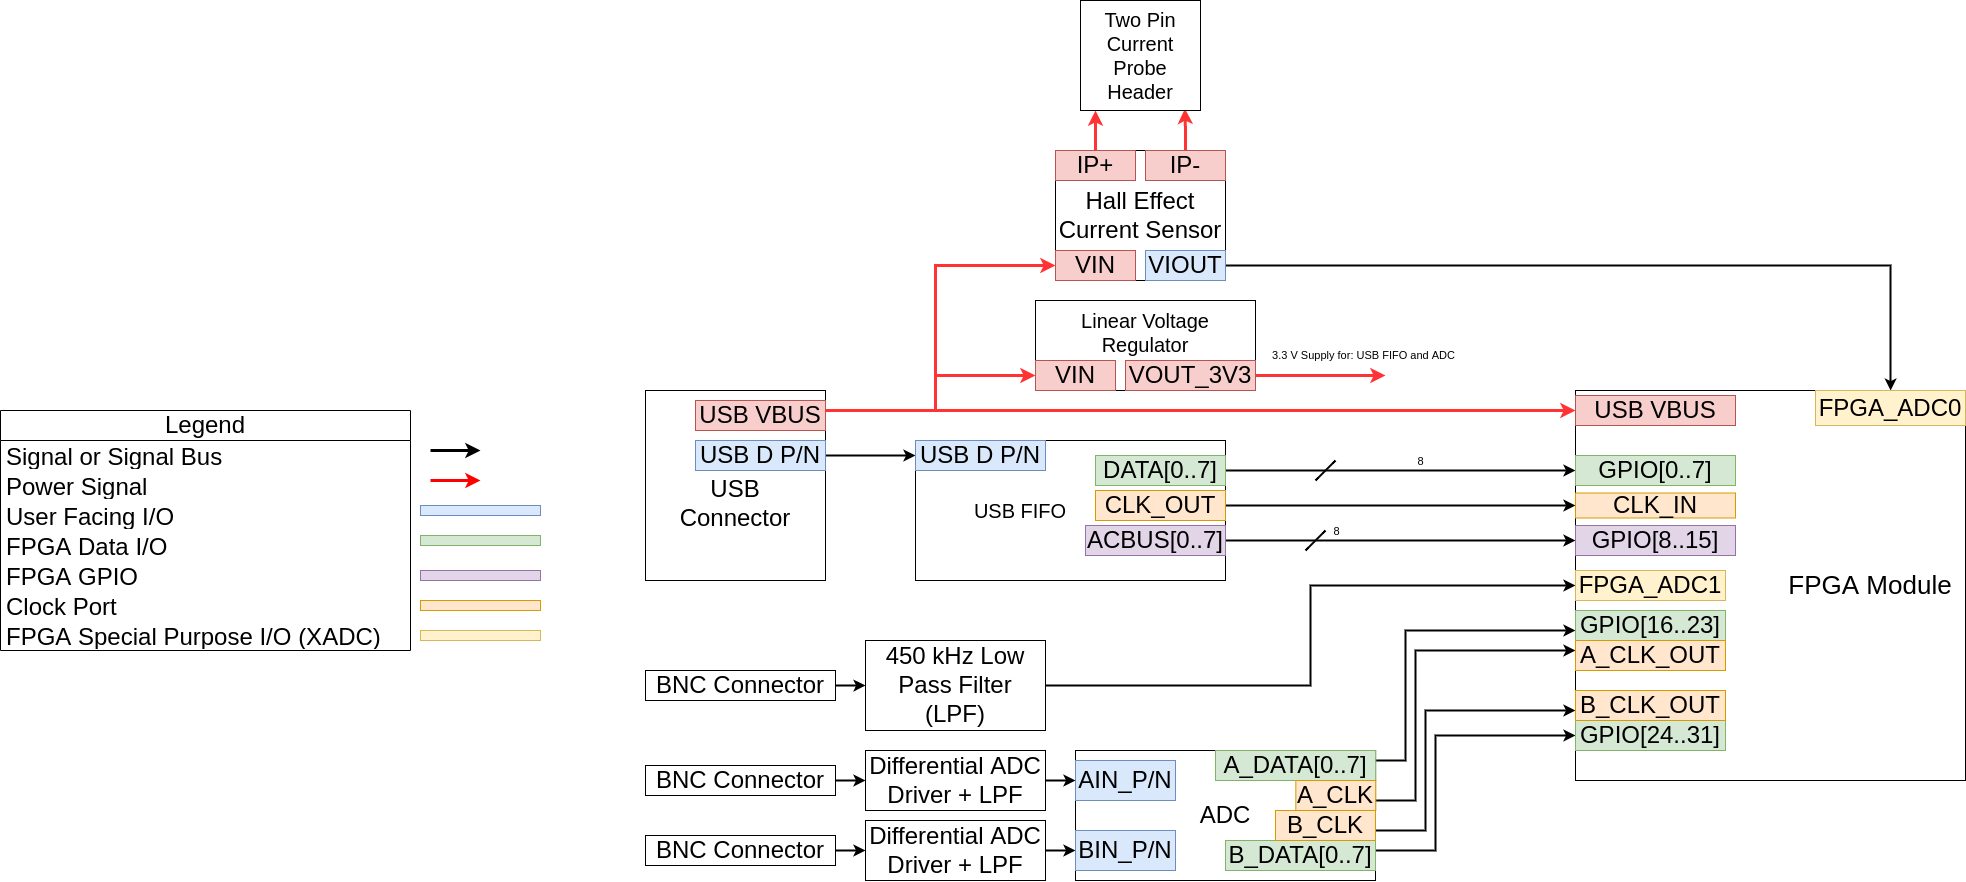
\includegraphics[width=\textwidth]{../../misc/TeachEE-System-Diagram-Hardware.png}
  \caption{Hardware System Block Diagram}
  \label{fig:hw-block-diagram}
\end{figure}

\subsection{FPGA} % Ethan
The FPGA RTL is driven by the implicit requirement to send multiple streams of
data with low latency. The sample rate and bandwidth requirements are not as
concerning in the design of the FPGA subsystem. This is because sample rates can
be easily tuned in the FPGA with clock generation PLLs and bandwidth depends on
the analog bandwidth of the input circuitry on the PCB.

In order to transmit multiple streams, the FPGA needs to frame multichannel
data in a standard packet format. A multiplexer is also used in the case that
sending all data at once oversaturates USB 2.0. With these issues
in mind, the diagram given in Figure \ref{fig:fpga-block-diagram} provides a
system-level block diagram for the FPGA design.

\begin{figure}[H]
  \centering
  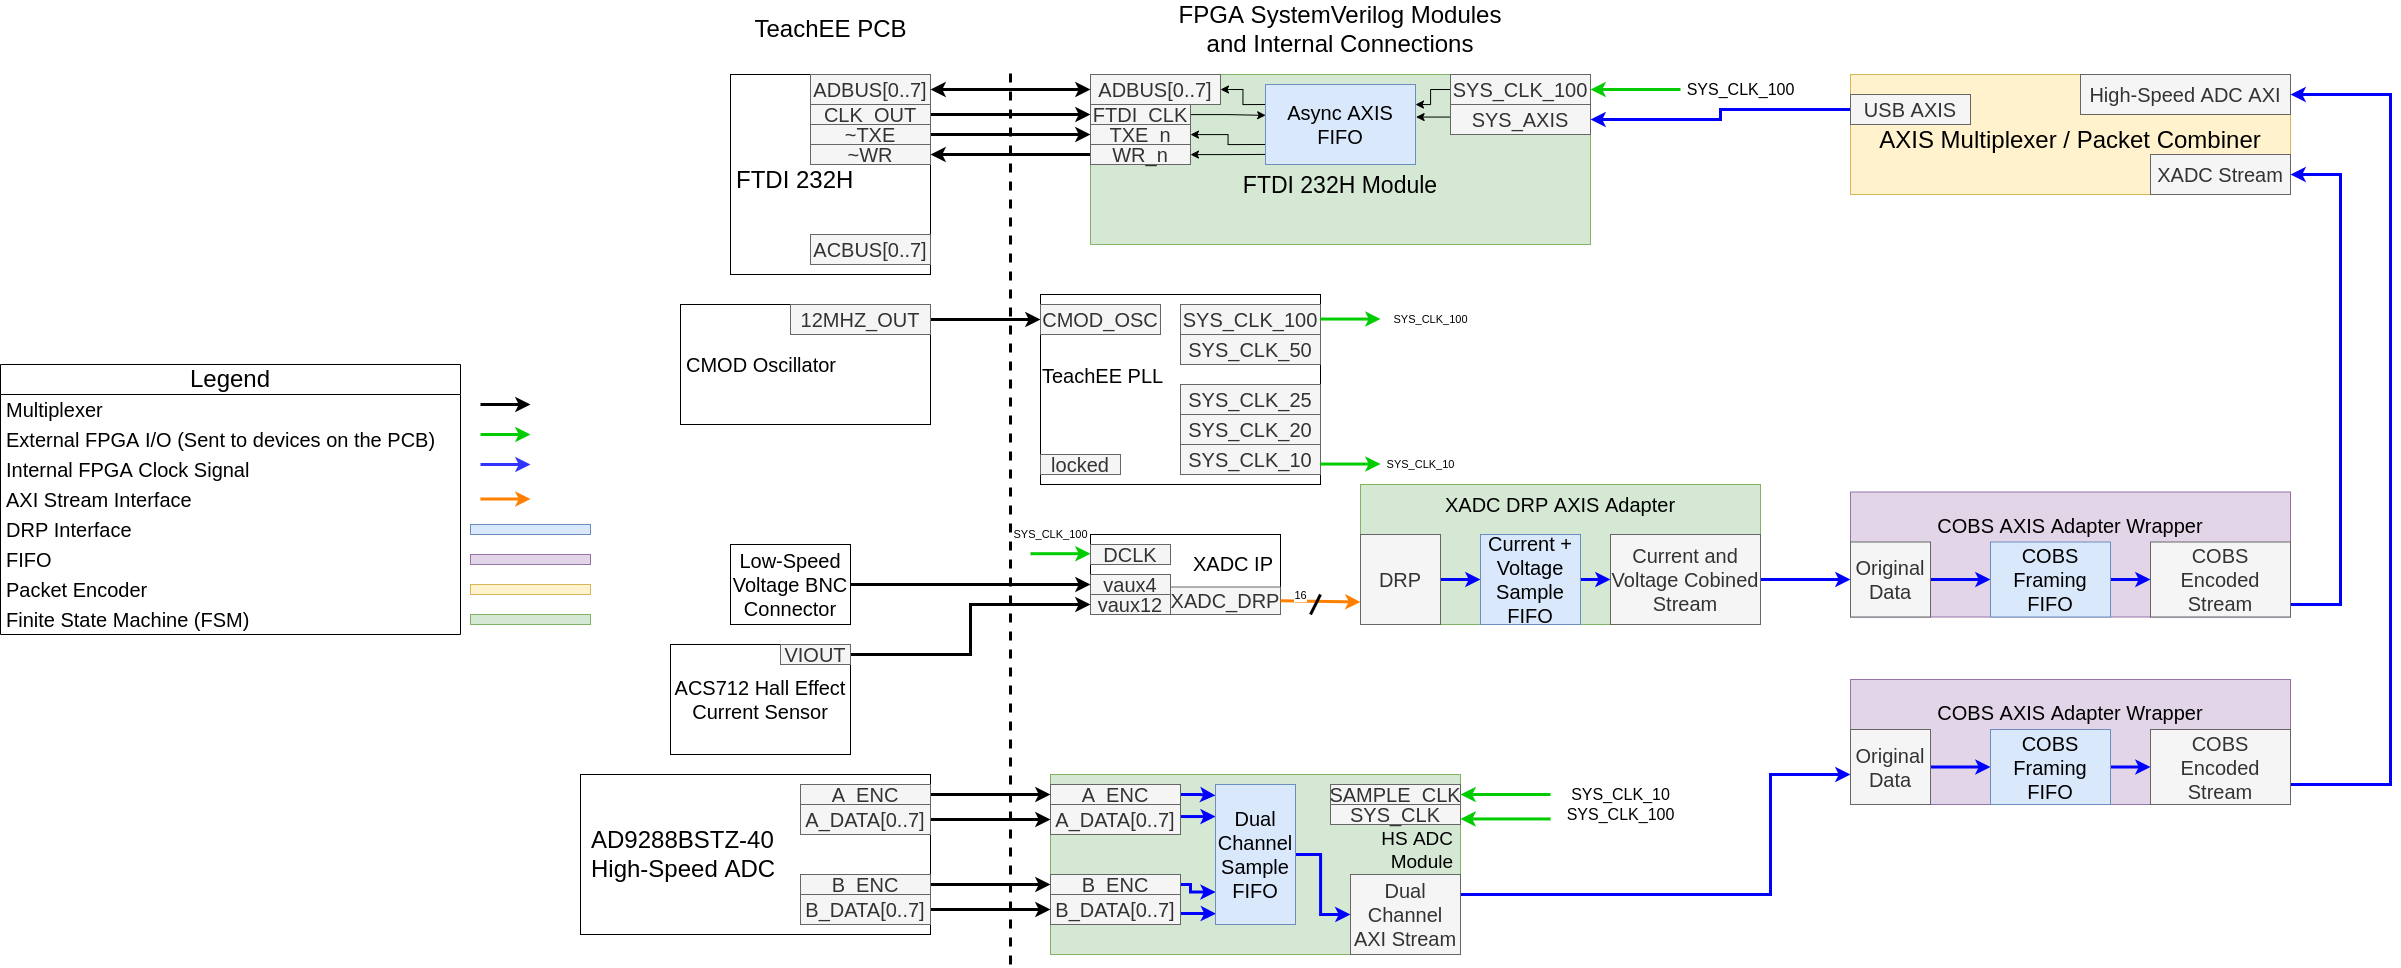
\includegraphics[width=\textwidth]{../../misc/TeachEE-System-Diagram-FPGA.png}
  \caption{FPGA System Block Diagram}
  \label{fig:fpga-block-diagram}
\end{figure}

A full breakdown of Figure \ref{fig:fpga-block-diagram} is given in Section
\ref{sec:impl} focusing on implementation. Overall, the initial design is nearly
identical to the final implementation. The team made use of COBS packet encoding
as promised in the blueprint and added a standard AXI Streaming protocol for the
internal FPGA datapath.

\subsection{Software} \label{sec:soft-design}% Tim
% Initial design: Tauri, two threaded one buffer guarded with mutex
% Stuff from blueprint with more detail (and from ECE night)

Several iterations were required to complete TeachEE's desktop application.
Initially, the prototype was built using the Tauri GUI framework. Tauri was
selected since it uses an instance of the Chrome Web Browser to render the user
interface, allowing developers to take advantage of the rich library and
tooling ecosystem for frontend web development. Despite these benefits, two
major factors necessitated a change: 1) displaying a rapidly changing
waveform using HTML and JavaScript at the required \SI{60}{\hertz} frame rate
proved extremely difficult; 2) data transfer between Rust and JavaScript
resulted in increased code complexity.

\code{egui} was selected as a replacement for Tauri because of its simple API
and large built-in widget library. \code{egui} is an \emph{immediate mode}
GUI, meaning it re-renders all widgets on every frame, regardless of whether or
not the application state had changed. This technique sacrifices
efficiency for a simpler programming model in which a developer expresses their
GUI as a single pure function \(f:~\text{State}~\mapsto~\text{UI}\)
\cite{egui}. An \emph{immediate mode} GUI is a good fit for TeachEE, since its
UI changes frequently and independently of user-input, nullifying the
aforementioned efficiency problem; even with a traditional \emph{retained mode}
GUI, widgets would still re-render whenever a new voltage/current is received.

Later in the software design process, performance issues were encountered
related to processing the incoming data stream fast enough to update the GUI at
\SI{30}{\hertz}. The slowdown was caused by the original threading model, in
which the USB Manager and App threads communicated via a single
shared buffer protected by a mutex. When the App thread attempted to
render a new frame, it would frequently be blocked by the USB Manager, which
was simultaneously writing incoming samples. The frequency and duration of this
blocking behaviour was prevalent enough to greatly reduce frame rate. To address
this problem, the software was reimplemented using the three thread
design described in Section \ref{sec:software-impl}.

\section{Implementation} \label{sec:impl}
%% Describe how the solution was implemented – this may involve a description of
%% major code blocks, schematics, photographs, CAD drawings, etc. The reader
%% should understand the materials and operation of your implemented project,
%% and the tools (hardware and/or software) used. This should also include a
%% full bill of materials and final project budget.

% Discuss how everything was implemented here
% Ethan will include figure of top level altium schematic
% Ethan will also include snippet of the top level SystemVerilog Module.
% I will pull in full schematics, layout and code into the appendices

The implementation is broken up into three subsections corresponding to each
subsystem.

\subsection{Hardware} % ETHAN
The hardware solution for TeachEE is implemented in the form of a four-layer
PCB. The PCB is designed using the EDA CAD software Altium Designer,
the industry standard tool for PCB design. Our design takes advantage of
Altium's hierarchical schematics. This allows the schematic to be broken up into
multiple pages with interconnects between the different sub-circuits.
TeachEE's top level schematic is an interconnect between all the sub-circuits of
the PCB, and is shown in Figure
\ref{fig:hw-top-level-sheet}. All eight pages of the
schematic are provided in Appendix \ref{appendix:schematic}.

\begin{figure}[H]
  \centering
  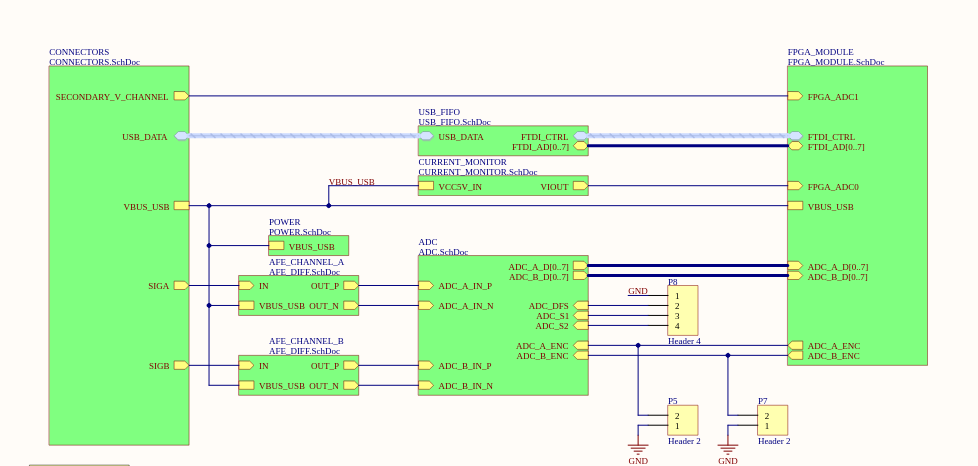
\includegraphics[width=\textwidth]{figures/altium-top-level.png}
  \caption{TeachEE PCB Top Level Schematic}
  \label{fig:hw-top-level-sheet}
\end{figure}

The following subsections break down each sub-circuit sheet entry in Figure
\ref{fig:hw-top-level-sheet}.

\subsubsection{Power}
The power schematic sheet contains a single LD1117V33C linear voltage regulator.
The regulator takes the \SI{5}{\volt} VBUS supply from the USB connection and
provides a \SI{3.3}{\volt} power output. A linear voltage regulator is employed
over a switching buck converter for the following reasons:
  \begin{enumerate}
    \item The analog to digital converters require clean voltage references to
      produce accurate readings and function correctly. Buck converters
      typically have noisier outputs that could harm performance.
    \item The linear voltage regulator requires fewer components to implement,
      easing chip shortage concerns.
    \item The significantly lower efficiency of a linear regulator is not an
      issue as this regulator has a capacity of \SI{1}{\ampere}, which is more
      than enough to run the devices on board.
  \end{enumerate}

\subsubsection{USB FIFO}
The USB FIFO is a queue that sends data out to the laptop over USB 2.0 Full
Speed (FS), capable of up to 480 Mbps. This circuit takes a
parallel byte stream from the FPGA and converts it to a USB 2.0 data stream. The
FT232HQ USB FIFO made by FTDI is used to implement this functionality. This chip
was selected over other USB Interface ICs for the following reasons:
  \begin{enumerate}
    \item Availability. USB Interfaces are one of many ICs in short supply
      in the ongoing chip shortage. In fact, this IC was ordered for the
      project after ELEC390 in July 2021 and only received in August 2022.
    \item Extensive preexisting software tooling. FTDI provides a driver and
      configuration utility for extracting data from their USB interfaces. This
      significantly reduces the software development work required to build a
      sample streaming interface. This ease of use is critical in a project with
      such a short timeline.
  \end{enumerate}

For debugging and circuit visibility, all digital control signals on the
FT232HQ are connected to test points. The schematic sheet also contains some
surrounding circuitry in the form of power filtering, a clock oscillator, and
configuration EEPROM.

\subsubsection{Current Monitor}
The current monitor page contains a hall effect current sensor circuit. The
circuit uses the ACS720KLATR current sensor. This sensor was chosen due
to its supply chain availability and the fact that it reports its reading
through a voltage output. The voltage output is linearly proportional to the
current flowing through the sensor plus a DC offset. This is a preferable
interface as it can be connected to an ADC channel without having to write
a new driver for the specific sensor on the FPGA. As such, the output of
the current sensor is connected to FPGA\_ADC0, which is one of two ADC channels
available on the FPGA module.

\subsubsection{ADC}
The TeachEE ADC schematic sheet contains an AD9288BSTZ dual channel
\SI{40}{\mega\samplepersec} ADC. This chip provides two additional high-speed
voltage channels in addition to the ADC channels provided by the FPGA
module. The data outputs for channels A and B are sent to the FPGA along
with the sample clocks. This ADC was selected for its FPGA friendly control
interface. Since the control consists of only a data bus and sample clock, it is
trivial to write an FPGA module to collect the data in comparison to other SPI
and I2C based converters on the market.

Bypass capacitors and ferrite beads are used to power the ADC for the cleanest
reference voltage possible. Additionally, the PCB contains non-populated
footprints for low pass filters, and filter bypasses to simplify testing and
debugging. For the digital side, all data busses and clocks have test points so
multimeters or oscilloscopes can be connected to debug the FPGA control signals.

\subsubsection{Analog Front End (AFE)}
The Analog Front End (AFE) sits in front of the inputs of the high-speed ADC. As
a result, this sub-circuit is duplicated twice in the top level sheet shown in Figure
\ref{fig:hw-top-level-sheet} to cover both channels. The AFE serves the following
purposes in the data acquisition hardware.

\begin{enumerate}
  \item Protect the ADC from over-voltage conditions. The front-end must clamp
    any voltages that would otherwise destroy the ADC.
  \item Convert the signal from single ended to differential. The ADC takes in a
    differential input, so the AFE must convert the input voltage observed at
    the connector to a differential signal of equivalent magnitude.
\end{enumerate}

This functionality is implemented in hardware using an AD8138 differential ADC
driver. This all-in-one component takes care of voltage clamping and
single-to-differential conversion. Moreover, it has sufficient analog bandwidth
to avoid reducing the effective bandwidth of the ADC. For debugging, the
sub-circuit contains 0-ohm bypass resistors that can be optionally soldered to
send the unclamped signal directly to the ADC.

\subsubsection{FPGA Module}
The FPGA module is implemented using a CMOD A7-35T Xilinx Spartan 7 Breakout
Board. It is connected to the PCB via two 28-pin headers. Two pins are
used for power and ground while the rest are used for FPGA IO pins. The USB FIFO
and ADC control pins are connected to the FPGA IO. There are also two special pins
which can be used as ADCs. These two pins are used to implement the current and
voltage channels at 1MSPS. The current sensor output is wired to one of the
channels and a BNC connector is connected to the other through a low pass filter
for voltage sampling.

The FPGA module schematic had one mistake that was not discovered until the
physical PCBs had already been manufactured and delivered. To use the
parallel-bus interface of the FT232HQ to send data, the FPGA must lock to a
\SI{60}{\mega\hertz} output clock from the FT232HQ. During layout, the FPGA
pin wired to this clock was swapped to a normal GPIO pin rather than an MRCC
dedicated clock pin. As a result, the FPGA place and route was failing during
compilation, as the FPGA could not route this clock from a standard GPIO pin.
This issue was resolved by waiving the warnings and optimizing the SystemVerilog
code to still pass timing without a proper clock route for the
\SI{60}{\mega\hertz} signal. Further information on this process is given in
Section \ref{sec:fpga-impl}.

\subsubsection{Connectors}
% Talk about LPFs and BNC connectors 
The connectors page contains all the external IO connections for TeachEE.
Specifically, the USB mini connector for data and three BNC connectors for scope
probes. The current sensor is exposed on its own separate pin header. The BNC
connectors are connected to the appropriate ADC input or AFE. Also, each
connector has the appropriate low pass filters to satisfy Nyquist's theorem. Each
connector also includes all the standard capacitors and resistors needed to
connect an oscilloscope probe from the lab kit sold at the Queen's bookstore.
\subsection{FPGA} \label{sec:fpga-impl} % ETHAN
% Refer to system block diagram and go module by module.
% put in the top level module code and some critical state machines
% Talk about AXIS as a standard protocol. Also the extensible to ARM SOCs it
% provides

The FPGA datapath and implementation can be summarized by examining the
interconnections between modules in the top level SystemVerilog module. Below is
each section of the top level TeachEE RTL module broken down and explained. The
entire RTL codebase can be viewed in Appendix \ref{appendix:rtl-code}.

\subsubsection{Top Level Module Interface}
Given below is the interface to the top level module of the TeachEE RTL code.

\setstretch{1}
\begin{minted}{systemverilog}
module teachee (
  input  var logic cmod_osc, // 12 MHz provided on the CMOD
  input  var logic ftdi_clk, // 60 MHz provided by the FTDI

  // FTDI Control Interface
  input  var logic ftdi_rxf_n,
  input  var logic ftdi_txe_n,

  output var logic ftdi_rd_n,
  output var logic ftdi_wr_n,
  output var logic ftdi_siwu_n,
  output var logic ftdi_oe_n,

  output var logic[7:0] ftdi_data,

  // High Speed ADC IO Interface
  output var logic hsadc_a_enc,
  input var logic[7:0] hsadc_a,

  output var logic hsadc_b_enc,
  input var logic[7:0] hsadc_b,

  input var logic[1:0] xa_n,
  input var logic[1:0] xa_p,
  ...
);
\end{minted}
\setstretch{2}

As shown above, the FPGA takes in a \SI{12}{\mega\hertz} clock provided by an
external oscillator and the \SI{60}{\mega\hertz} clock from the FT232HQ. After
the clocks, IO for the FT232HQ and AD9288BSTZ control signals are defined. Some
additional pins spare pins and LED signals at the end of the interface
declaration are not shown as they were used for debugging purposes.

\subsubsection{PLL Clock Generation}
After the module interface is declared, the PLL system clock generator is
initialized. This is an IP core provided by the FPGA manufacturer Xilinx that
takes the oscillator \SI{12}{\mega\hertz} input and outputs a variety of useful
clock signals for the rest of the design. Given below is the IP core module
instantiation.

\setstretch{1}
\begin{minted}{systemverilog}
    teachee_pll teachee_pll_ip_inst (
        // Clock out ports
        .clk_100(clk_100),     // output clk_100
        .clk_50(clk_50),     // output clk_50
        .clk_25(clk_25),     // output clk_25
        .clk_20(clk_20),     // output clk_20
        .clk_10(clk_10),     // output clk_10

        // Status and control signals
        .reset(0), // input reset
        .locked(locked),       // output locked

        // Clock in ports
        .cmod_osc(cmod_osc)      // input cmod_osc
    );
\end{minted}
\setstretch{2}

The module takes the external oscillator clock as an input and outputs 100, 50,
25, 20 and \SI{10}{\mega\hertz} clocks. Different frequencies can be specified
within the Xilinx Vivado IDE used to flash the FPGA. In the current
implementation, only the 100 and \SI{10}{\mega\hertz} clocks are used.
\SI{100}{\mega\hertz} is used throughout the top level system and
\SI{10}{\mega\hertz} is used as a sampling clock in the high speed ADC. One
clock that is not covered by this PLL is the \SI{60}{\mega\hertz} clock
generated externally by the FT232HQ. The PLL also has a \code{locked} output.
When driven high, this signal indicates that the PLL is locked to the input
clock and the output clocks are functioning correctly. This signal is used to
send a reset signal to all modules, holding them in reset until the PLL has
locked and all clocks are up and running.

\subsubsection{Interface Instantiations} \label{sec:interface-inst}

Given below are the instantiations for the different interfaces used to make
connections between the submodules. Interfaces in SystemVerilog can be thought
of as groupings of wires that make managing inter-module connections easier as
each wire does not need to be explicitly declared.

\setstretch{1}
\begin{minted}{systemverilog}
    hsadc_interface hsadc_ctrl ();
    ...
    axis_interface #(
        .DATA_WIDTH(2 * XADC_DRP_DATA_WIDTH)
    ) xadc_sample_channel (
        .clk(sys_clk),
        .rst(reset)
    );

    axis_interface #(
        .DATA_WIDTH(16)
    ) hsadc_sample_channel (
        .clk(sys_clk),
        .rst(reset)
    );
\end{minted}
\setstretch{2}

The first interface declared is for the AD8138ARZ high-speed ADC. External IO
signals are assigned to the different control wires in the interface. Next, the
various AXIS interfaces required to connect the modules are instantiated. The
interface width is specified using the \code{DATA_WIDTH} parameter. 8-bit
interfaces are used to connect the packet stream output for a given ADC to the
FT232HQ wrapper module that adapts the AXI Stream to FT232HQ control signals.
The remaining two interfaces hold the sample data from the XADC and high-speed
ADC respectively. The XADC is the dual channel 16-bit ADC built into the FPGA.
The two sample data interfaces \code{hsadc_sample_channel} and
\code{xadc_sample_channel} are each connected to the outputs of adapter modules
that adapt the native interface of the device to an AXI Stream. The AXI Stream
interface used is a custom wrapper for all the standard signals found in an AXI
stream. The interface definition can be found in Appendix
\ref{appendix:axis-interface}.

The AXIS Protocol, also known as AXI Stream, is derived from ARM's AXI bus
specification. Additional information on the AXI Stream protocol and the
external libraries used to support it can be found in Section
\ref{sec:external-fpga-libs}.

\subsubsection{FT232HQ AXIS Wrapper}
After instantiating the interfaces, they are used to make connections between
the various submodules. Shown below is the \code{ft232h} module instance used
to send data to the computer over USB.

\setstretch{1}
\begin{minted}{systemverilog}
    ft232h usb_fifo (
        .ftdi_clk(ftdi_clk),

        .ftdi_rxf_n(ftdi_rxf_n),
        .ftdi_txe_n(ftdi_txe_n),

        .ftdi_rd_n(ftdi_rd_n),
        .ftdi_wr_n(ftdi_wr_n),
        .ftdi_siwu_n(ftdi_siwu_n),
        .ftdi_oe_n(ftdi_oe_n),

        .ftdi_adbus(ftdi_data),

        // Programmer AXIS Interface
        // CHANGE THIS BASED ON WHETHER YOU WANT TO USE XADC OR HSADC
        .sys_axis(xadc_usb_axis.Sink)
    );
\end{minted}
\setstretch{2}

This module consists of a state machine that adapts the AXI Stream of sample
packets to control signals of the FT232HQ. The input is the \code{sys_axis}
stream and the output is all the \code{ftdi_*} control signals used to produce
data over USB. Wrapping the FT232HQ interface in a standard AXI Stream makes it
trivial to interface with all the other modules in the TeachEE source code. The
same design approach is used throughout the codebase to ensure compatibility
between the various hardware interface modules. The state machine for the module
is shown in Figure \ref{fig:ft232h-state-machine}.

\begin{figure}[H]
  \centering
  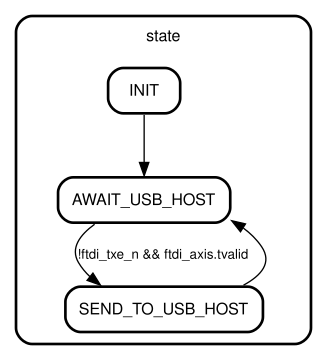
\includegraphics[width=\textwidth/3]{figures/ft232h-state-machine.png}
  \caption{FT322H AXI Wrapper State Machine}
  \label{fig:ft232h-state-machine}
\end{figure}

The state machine waits for the AXI Stream to have data available and for the
FT232HQ to be ready for new data. When this condition is satisfied, the byte is
sent out and the state machine automatically transitions back to the await
state.

Regarding the comment in the code above about changing the \code{sys_axis}
stream input, in this case, the XADC is used.

\subsubsection{XADC IP Core}
Shown below is the XADC IP core used to extract data from the internal XADC on
the FPGA. This IP core is made custom using the XADC Wizard tool in Xilinx
Vivado. The core is configured to only output the two FPGA ADC channels in use
on the TeachEE PCB via a Dynamic Reconfiguration Port (DRP) interface. The DRP
signals are then fed into an AXIS adapter module for interface standardization.

\setstretch{1}
\begin{minted}{systemverilog}
    xadc_teachee xadc_teachee_inst (
        // Clock and Reset
        .dclk_in(sys_clk),          // input wire dclk_in
        .reset_in(reset),        // input wire reset_in

        // DRP interface
        .di_in(0),              // input wire [15 : 0] di_in
        .daddr_in(xadc_daddr),        // input wire [6 : 0] daddr_in
        .den_in(xadc_den),            // input wire den_in
        .dwe_in(0),            // input wire dwe_in
        .drdy_out(xadc_drdy),        // output wire drdy_out
        .do_out(xadc_do),            // output wire [15 : 0] do_out

        // Dedicated analog input channel (we do not use this)
        .vp_in(0),              // input wire vp_in
        .vn_in(0),              // input wire vn_in

        // analog input channels, vaux4 is pin 15 = VIOUT of current sensor
        // vaux12 is pin 16 = low speed voltage channel.
        .vauxp4(xa_p[0]),            // input wire vauxp4
        .vauxn4(xa_n[0]),            // input wire vauxn4
        .vauxp12(xa_p[1]),          // input wire vauxp12
        .vauxn12(xa_n[1]),          // input wire vauxn12

        // conversion status signals
        .channel_out(),  // output wire [4 : 0] channel_out
        .eoc_out(),          // output wire eoc_out
        .alarm_out(),      // output wire alarm_out
        .eos_out(xadc_eos),          // output wire eos_out
        .busy_out()        // output wire busy_out
    );
\end{minted}
\setstretch{2}

\subsubsection{ADC AXIS Wrappers}
Similarly to the \code{ft232h} module, both the XADC and high-speed ADC have
AXIS wrapper modules. Both wrapper modules function in the same manner, they
await new data from the ADC and place it in AXIS compliant FIFO queues. The
\code{sample_stream} output is internally connected to this queue where samples
can be consumed by the FT232HQ. Given below is the instantiation of both
modules.

\setstretch{1}
\begin{minted}{systemverilog}
    xadc_drp_addr_t xadc_daddr;
    var logic xadc_den;

    var logic xadc_drdy;
    var logic[XADC_DRP_DATA_WIDTH-1:0] xadc_do;
    var logic xadc_eos;

    xadc_drp_axis_single_stream xadc_drp_axis_adapter_inst (
        .xadc_dclk(sys_clk),
        .xadc_reset(reset),

        // DRP and Conversion Signals
        .xadc_daddr(xadc_daddr),
        .xadc_den(xadc_den),
        .xadc_drdy(xadc_drdy),
        .xadc_do(xadc_do),

        .xadc_eos(xadc_eos),

        .sample_stream(xadc_sample_channel.Source)
    );

    hsadc_axis_wrapper hsadc (
        .sample_clk(clk_10),
        .stream_clk(sys_clk),
        .reset(reset),

        .hsadc_ctrl_signals(hsadc_ctrl.sink),
        .sample_stream(hsadc_sample_channel.source)
    );

\end{minted}
\setstretch{2}

The XADC wrapper takes in the DRP control signals from the XADC IP core and the
high-speed ADC wrapper gets all the control signals from a single interface
declared earlier in the file.


\subsubsection{AXIS and Verilog AXIS} \label{sec:external-fpga-libs} AXIS, also
referred to as AXI Stream, is the standard protocol used throughout the FPGA
datapath. While there are many signals in an AXI interface, the primary signals
are called \code{tdata}, \code{tready}, and \code{tvalid}. Only when \code{tready}
and \code{tvalid} are asserted can data be consumed from the \code{tdata} bus.
\code{tready} is controlled by the receiver so that it can regulate the rate at which
it consumes data, while \code{tvalid} is controlled by the sender to notify the
receiver when new data is ready on the \code{tdata} lines. The full
specification contains many additional signals, but these three are the ones most
often manipulated during data transmission \cite{axis_spec}. Figures
\ref{fig:axis-read} and \ref{fig:axis-write} show the AXIS read and write timing
diagrams respectively.

\begin{figure}[H]
  \centering
  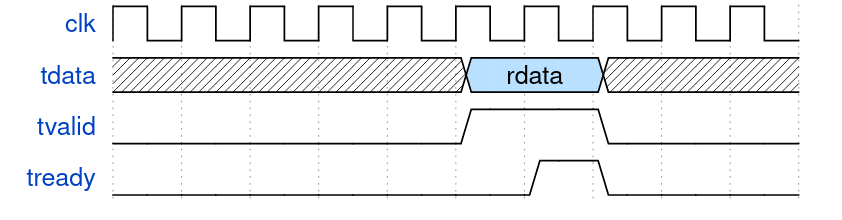
\includegraphics[width=\textwidth]{figures/axis_read.png}
  \caption{AXIS Read Transaction Timing Diagram}
  \label{fig:axis-read}
\end{figure}

In AXIS read and write transactions, the producer is responsible for
\code{tdata} and \code{tvalid} signals while the consumer toggles \code{tready}.
This allows the consumer to know when new data becomes available and it is able
to signal to the producer when it is ready to accept it via \code{tready}. All
three signals should only be asserted or deasserted in synchronization with the
system clock, as per the specification. As shown in Figure \ref{fig:axis-read},
\code{tvalid} is asserted on the same rising edge as the new data coming onto
the \code{tdata} bus. The consumer sees this and asserts tready on the next
rising edge consuming the data. In the case where multiple words of data are
queued by the producer, the \code{tdata} value will advance to the next byte
available after each cycle where both \code{tvalid} and \code{tready} are true. This
allows a new read to take place every cycle if the producer has the data and the
consumer is ready for it. This simple protocol yields strong performance and
flexibility with minimal FPGA LUT resources used. It should be noted that for
any AXIS transaction to take place \code{tready} and \code{tvalid} must both be true.

\begin{figure}[H]
  \centering
  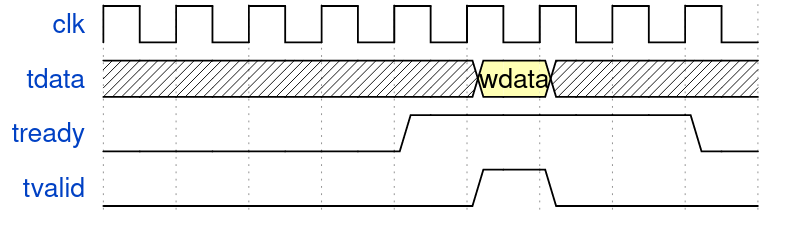
\includegraphics[width=\textwidth]{figures/axis_write.png}
  \caption{AXIS Write Transaction Timing Diagram}
  \label{fig:axis-write}
\end{figure}

In the AXIS write case shown in Figure \ref{fig:axis-write}, the consumer first
asserts \code{tready}, which tells the producer that it can accept new data.
Once the producer has data, it asserts the value on \code{tdata} and drives
\code{tvalid} high on the same rising edge. Since \code{tready && tvalid} is
true, the data is written to the consumer successfully. This design pattern is
replicated repeatedly throughout the FPGA codebase provided in Appendix
\ref{appendix:rtl-code}.

In addition to the simplicity of the protocol, there is significant library support for
AXI Streams. In the case of TeachEE, the \code{verilog-axis} library is used
\cite{verilog_axis_lib}. This library contains a variety of useful Verilog
modules, all of which expose an AXIS interface at their inputs and outputs. The
standard interface across all modules trivializes connecting up the library modules
with TeachEE modules. The only modification made to these library
modules was to wrap them in another more ergonomic module. Since the library is
written in Verilog, it does not have access to interfaces, which are a feature
of SystemVerilog only. As a result, each AXIS signal is written out individually
making instantiating and connecting the modules unwieldy. To bundle all
these signals into one module port, the \code{axis_interface} is used. For each
module in the \code{verilog-axis} library used by TeachEE, a wrapper module is
written that places all the signals for the AXI Streams in AXIS interfaces,
making module connectivity far simpler with SystemVerilog. This is possible
due to the Xilinx Vivado project build configuration that cross compiles both
Verilog and SystemVerilog. The interface is also designed to seamlessly handle
the producer and consumer cases discussed above using modports. The
\code{Source} modport can be used on producer stream interfaces and the
\code{Sink} modport can be used for consumers. The modports switch the direction
of the signals from \code{input} to \code{output} depending on the use case.

\code{verilog-axis} contains many modules but there are three that were employed
when writing the RTL code for TeachEE. 

The first module is \code{axis_async_fifo}, which is wrapped by
\code{axis_async_fifo_wrapper}. This module constructs a First-In-First-Out
(FIFO) Queue and is used repeatedly throughout the code. The first and foremost
purpose of the Queue is to provide sample memory to ensure samples are not
dropped when the rate of production deviates from the rate of consumption.
Secondly, the FIFO is asynchronous, meaning it can use different clock signals
for its input and output. The module has internal synchronization logic to bring
data across clock domains. This functionality was critical in the TeachEE RTL
design as there were multiple clock domains that needed efficient data transfer between
them. The top-level system, USB FIFO, HSADC, and XADC all had different
clock signals and had their data inputs buffered by asynchronous FIFOs.

The second key module is the \code{axis_adapter}, which is wrapped by
\code{axis_adapter_wrapper}. This module takes an AXI Stream and adapts it to a
smaller width specified as a parameter in the module instantiation. This module
was critical in getting the 32-bit sample stream from the XADC to fit the 8-bit
stream accepted by the USB FIFO.

The final module used from the library was \code{cobs_encode}, which is
wrapped by \code{cobs_encode_wrapper}. This module takes an 8-bit input stream
and outputs the same data encoded using Consistent Overhead Byte Stuffing
(COBS). The COBS encoder is highly efficient and only creates two additional
bytes of overhead, minimizing USB link bandwidth wastage \cite{cobs}.
To transmit samples to the computer, the 32-bit stream from the XADC
(or 16-bit from the HSADC) is adapted to 8 bits using \code{axis_adapter}. The
resulting 8-bit stream is fed into the COBS encoder, whose output is connected
to the USB FIFO. These two modules make up the packet encoding stack.

Perhaps the most important benefit of AXIS over other streaming interfaces is
its direct compatibility with the more fully-featured AXI bus. AXI is a standard
memory-mapped bus interface used in ARM processors \cite{axi_spec}. Since all
modules in TeachEE's FPGA codebase use AXI Streams, the platform is highly
extensible and can be connected to ARM coprocessors with minimal effort. Such a
design extension would make TeachEE architecturally similar to more expensive
benchtop oscilloscopes that make use of both an ASIC and traditional processor
through a high-speed interconnection protocol. An example of this architecture
is Keysight's MegaZoom ASIC \cite{keysight_megazoom}.

\subsection{Software} \label{sec:software-impl} % ERIC 
TeachEE's software workload is split between three modules, each of which runs in its
own thread. The first module is the USB Manager, responsible for reading and decoding
packets from the hardware driver. The second is the App, responsible for updating and
displaying the user interface. Finally, the Controller facilitates communication between
the two and provides additional sample processing.

The software for TeachEE follows an improved threading model described in
Figure \ref{fig:soft-sequence-diagram} below. This design change was necessitated
by software performance issues encountered in the initial design, described in
Section \ref{sec:soft-performance-issues}. The USB manager and Controller share one set of
two buffers, referred to as the USB Buffers, and the App and Controller share
another set of two buffers, the App buffers. The threads coordinate their workflows
such that each thread can exclusively operate on a buffer at a time. For example,
while the USB Manager is writing samples to USB Buffer 0, the Controller can copy
samples from USB Buffer 1 to App Buffer 1, and the App can read from App Buffer 0.
After every work cycle, each thread swaps to the other buffer. This protocol
parallelizes the workload as much as possible and minimizes thread block times.

\begin{figure}[H]
  \centering
  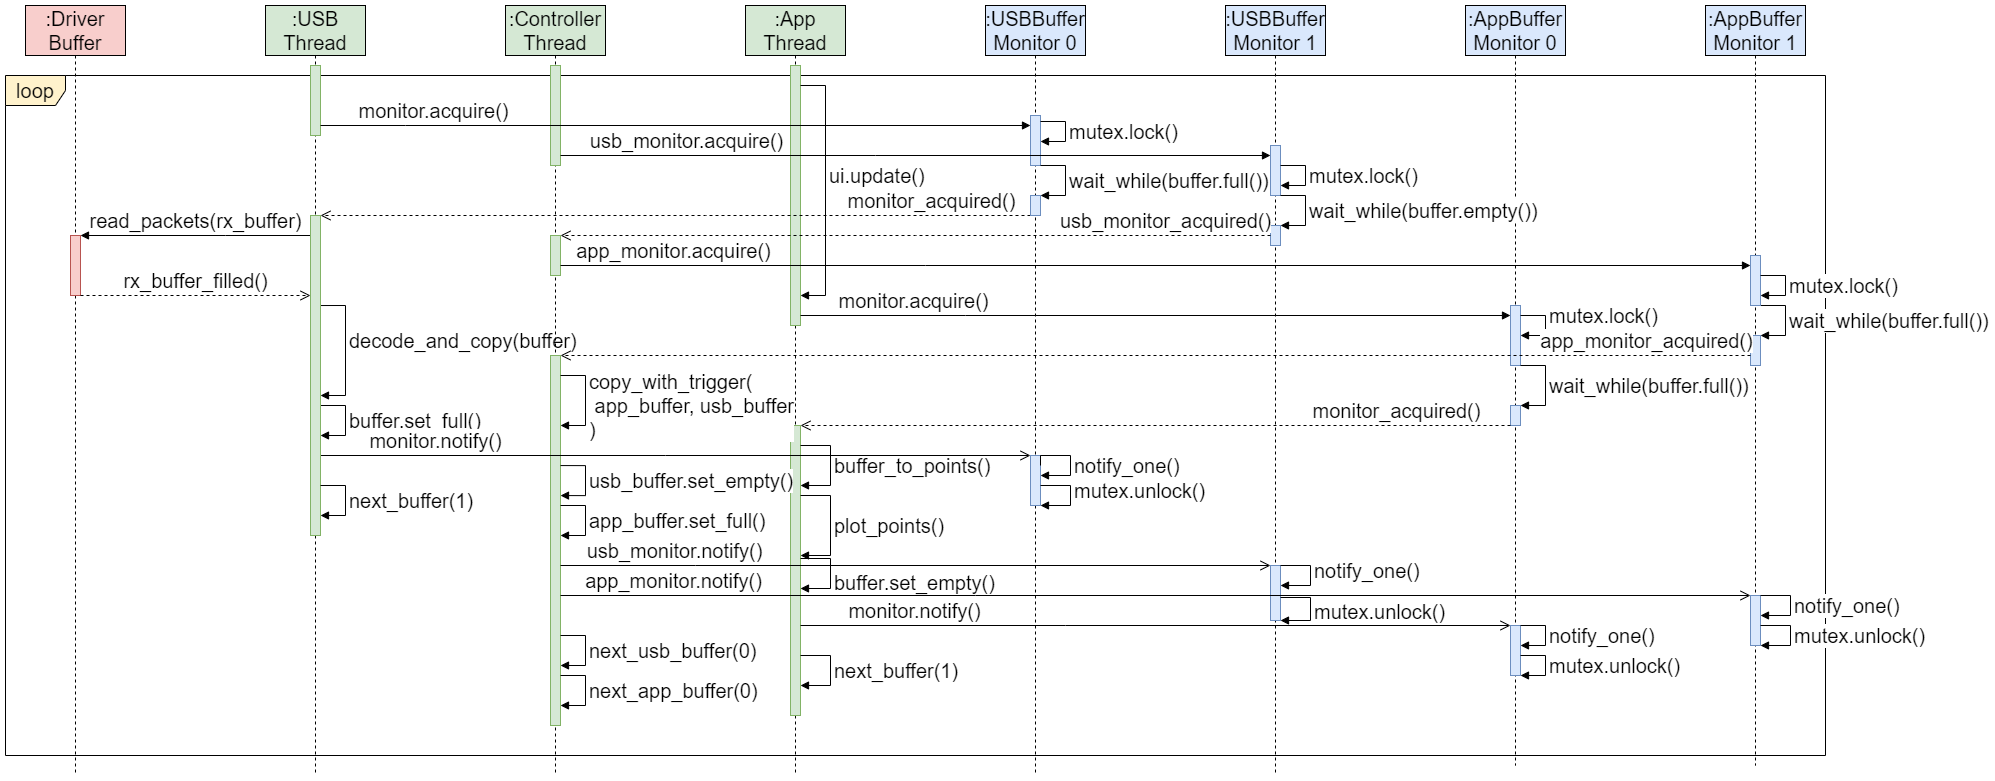
\includegraphics[width=\textwidth]{../../misc/sequence_diagram.drawio.png}
  \caption{Threading Model Sequence Diagram}
  \label{fig:soft-sequence-diagram}
\end{figure}

The sequence diagram above simplifies the buffer representation. Each buffer in the
two sets actually represents several buffers/channels in the \code{Channels}
struct. In the current implementation, two channels are supported and every buffer
operation operates on both channels simultaneously. Furthermore, each \code{Channels}
struct is wrapped in a \code{BufferState} enum, representing the emptiness/fullness
of the channels, which in turn is guarded by a monitor. To allow these monitors to
be shared between threads, they are wrapped by Rust's shared pointer, the \code{Arc}.
Figure \ref{fig:soft-buffer-config} below illustrates the shared data's configuration.
Note that there is an additional field in the \code{Channels} struct used to store the
results of frequency spectrum analysis performed in the Controller thread. This field
is unused in the USB Buffer \code{Channels}.

\begin{figure}[H]
  \centering
  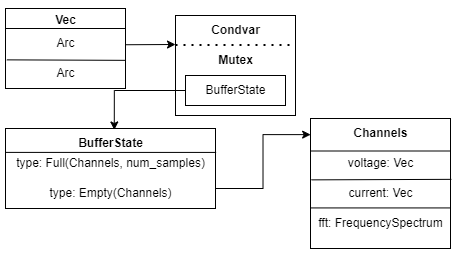
\includegraphics[width=8cm]{figures/buffer_config.drawio.png}
  \caption{Shared data configuration representing one set of ``buffers"}
  \label{fig:soft-buffer-config}
\end{figure}

In Rust, a monitor is implemented as a condition variable and mutex tuple. The condition
variable allows threads to wait while a condition is true. The mutex ensures that only
one thread is allowed access to a given \code{Channels} at a time. A thread acquires a
monitor by first locking the mutex. Once the mutex is locked, the thread checks the
\code{BufferState}. If the thread intends to write to the buffers, but the buffers are
\code{Full}, it unlocks the mutex and goes to sleep until it receives a notification
that the buffers have been emptied. The same applies to threads attempting to read from
\code{Empty} buffers. Once the thread is notified, it is woken from the wait function
with the mutex reacquired. A thread releases a monitor by setting the \code{BufferState}
to the appropriate type and notifies a thread waiting on the condition variable. The
mutex is unlocked implicitly when it goes out of scope. An example of this procedure
(run by the App thread) is given in the code block below.

\setstretch{1}
\begin{minted}{rust}
  // Wait until controller thread has filled the current buffer.
  let mut buf_state = condvar
      .wait_while(mutex.lock().unwrap(), |buf_state| buf_state.is_empty())
      .unwrap();
  // Get the Channels buffers.
  let (channels, num_samples) = buf_state.unwrap();
  ...
  // Release the monitor.
  *buf_state = BufferState::Empty(channels);
  condvar.notify_one();
\end{minted}
\setstretch{2}

\subsubsection{The USB Manager}
The USB Manager thread reads packets from the FTDI receiver queue into a buffer,
decodes them into voltage and current samples, and populates the USB Buffers.
The packets are read from the queue using an FTDI library. The thread always
reads 120 000 bytes at a time so that after decoding, the App displays
approximately 20 000 samples each cycle. This ensures that the plotted waveform
does not expand or contract in the horizontal direction, which improves the
user's experience.

The decoding function decodes the six-byte COBS packets into pairs of voltage
and current samples. The main decoding loop is described in the code below.

\setstretch{1}
\begin{minted}{rust}
  ...
  'outer: while src_index + PACKET_SIZE < end
      && dst_index < channels.voltage1.len()
  {
      // Packet error: offset byte not in [1, 5] or packet not delimited
      // with 0
      if self.rx_buf[src_index] == 0
          || self.rx_buf[src_index] >= PACKET_SIZE as u8
          || self.rx_buf[src_index + PACKET_SIZE - 1] != 0
      {
          // Find the next 0 and continue from there
      } else {
          let packet = &self.rx_buf[src_index..(src_index + PACKET_SIZE)];
          let mut block = packet[0] - 1;
          // Two bytes of packet overhead
          let mut decoded: [u8; PACKET_SIZE - 2] = [0; PACKET_SIZE - 2];
          let mut decoded_index = 0;

          // Note: the packet index is just the decoded_index + 1 (skip
          //       the first offset byte)
          // Example packet: 01 02 22 02 44 00
          // Decodes to:        00 22 00 44
          while decoded_index < decoded.len() {
              if block > 0 {
                  decoded[decoded_index] = packet[decoded_index + 1];
              } else {
                  decoded[decoded_index] = 0;
                  block = packet[decoded_index + 1];
              }
              decoded_index += 1;
              block -= 1;
          }

          // Map digital values with 4096 discrete levels to samples
          channels.voltage1[dst_index] =
              (((decoded[3] as u16) << 4) | decoded[2] as u16) as f64
                  * 3.3 / 4095.0;
          channels.current1[dst_index] =
              ((((decoded[1] as u16) << 4) | decoded[0] as u16) as f64
                  * 3.3 / 4095.0 - 1.5) * (1.0 / 0.09);
          src_index += PACKET_SIZE;
          dst_index += 1;
      }
  }
  ...
\end{minted}
\setstretch{2}

The full USB Manager code is provided in Appendix \ref{appendix:software-usb_manager}.

\subsubsection{The Controller} \label{sec:soft-controller}
The Controller thread copies samples from the USB Buffers to the App Buffers.
If enabled by the user, it also performs rising edge triggering and/or frequency
spectrum analysis on the samples. The triggering algorithm uses hysteresis to
find the first rising edge while ignoring rising edges from noise. It does this
by setting the hysteresis to 25\% of the signal peak-to-peak so that only larger
rising edges are triggered on \cite{hysteresis}. Triggering is done on both the
voltage and current channels with separate thresholds provided by the user.
The triggering function is provided below.

\setstretch{1}
\begin{minted}{rust}
    /// Returns position of first rising edge based on threshold
    fn hysteresis_trigger(src: &[f64], trigger: f64) -> usize {
        // Hysteresis width as fraction of peak to peak
        const HYSTERESIS_WIDTH: f64 = 0.25;
        let mut max_val = f64::MIN;
        let mut min_val = f64::MAX;
        for &val in src.iter() {
            max_val = f64::max(max_val, val);
            min_val = f64::min(min_val, val);
        }
        let hysteresis = (max_val - min_val) * HYSTERESIS_WIDTH;

        // Trigger when signal first falls below 'trigger - hysteresis'
        // and then rises above trigger
        let first_lower = src.iter().position(|&val| val < trigger -
            hysteresis);
        if let Some(lower_idx) = first_lower {
            let first_higher = src[lower_idx..].iter().position(
                |&val| val >= trigger);
            if let Some(higher_idx) = first_higher {
                return lower_idx + higher_idx;
            }
        }
        // Don't trigger if it failed
        0
    }
\end{minted}
\setstretch{2}

Spectrum analysis is performed using the \code{spectrum-analyzer} library. The
provided function takes the sample data, sample rate, desired frequency range,
and an optional scaling function and returns a \code{FrequencySpectrum} struct.
This struct contains an array of frequency/magnitude tuples, which can be passed
to the App to be displayed.

The full Controller code is provided in Appendix \ref{appendix:software-controller}
and includes the trigger and spectrum analysis procedures.

\subsubsection{The App}
\code{egui} is a simple and fast GUI library written entirely in Rust \cite{egui}.
It is an immediate mode GUI, which means that the UI is refreshed at approximately
sixty frames per second and does not require any event handlers. This makes it
ideal for writing simple and highly interactive UIs quickly as it eliminates the
need for complex callbacks, UI objects, or state storage. \code{egui} was chosen to
implement the front end for TeachEE instead of JavaScript to avoid the overhead of
message passing.

The function below adds and manages a pair of offset/scale sliders, and is an example
of the simplicity of the \code{egui} library. This function is called three times to
add the three pairs of sliders shown in Figure \ref{fig:soft-ui}.

\setstretch{1}
\begin{minted}{rust}
    fn offset_scale_sliders(
        ui: &mut Ui,
        offset: &mut f64,
        o_range: RangeInclusive<f64>,
        scale: &mut f64,
        s_range: RangeInclusive<f64>,
    ) {
        ui.columns(2, |uis| {
            uis[0].label("Offset");
            uis[0].add(Slider::new(offset, o_range).clamp_to_range(false));
            uis[1].label("Scale");
            uis[1].add(
                Slider::new(scale, s_range)
                    .clamp_to_range(false)
                    .logarithmic(true),
            );
        });
    }
\end{minted}
\setstretch{2}

The App stores two structs: an \code{AppData} and a \code{UIControls}.
\code{AppData} stores the App Buffers, trigger thresholds, and frequency spectrum
enable, and is shared with the Controller thread. \code{UIControls} stores the
current UI state set by the user, e.g., offsets, scaling, trigger thresholds, and
spectrum analysis enable/disable.

TeachEE implements several features reflected in the UI, including:
\begin{enumerate}
  \item Individual channel scaling and offsetting (both horizontal and vertical)
  \item Rising edge triggering with user-provided thresholds
  \item Signal plotting with cursor and various navigation options
  \item Plotting of signals in the frequency domain
  \item Exporting plotted signals to a CSV file
  \item Ability to turn individual channels on and off
\end{enumerate} 
Figure \ref{fig:soft-ui} shows all of TeachEE's features in use at the same time.

\begin{figure}[H]
  \centering
  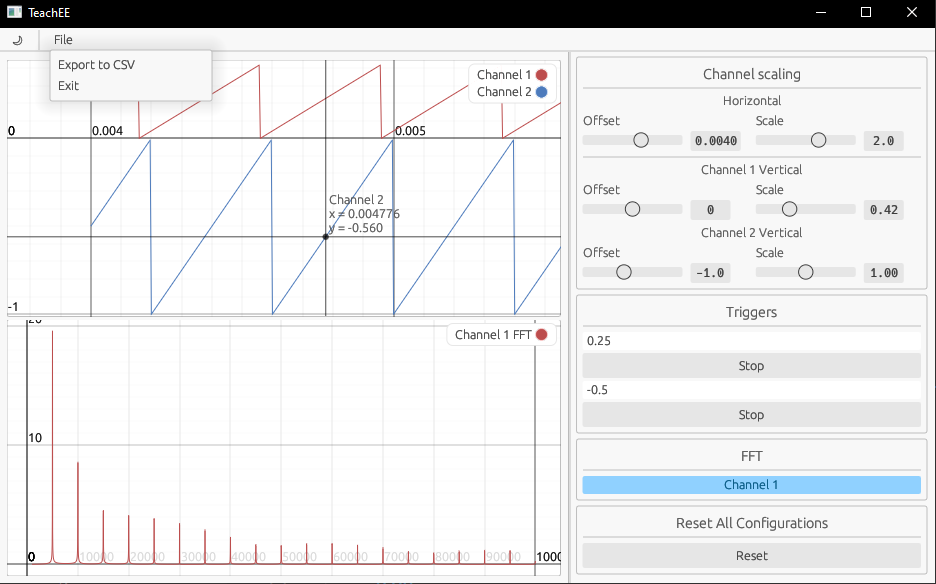
\includegraphics[width=\textwidth]{figures/software-ui.png}
  \caption{Example screenshot showcasing all UI features}
  \label{fig:soft-ui}
\end{figure}

The full App code is provided in Appendix \ref{appendix:software-app} and contains
the UI implementation.

\section{Testing, Evaluation \& Verification} \label{sec:testing}
The testing and validation of TeachEE consisted of testing the hardware/PCB,
FPGA, and software subsystems. The following subsections cover each subsystem of
TeachEE in full detail. Testing was performed in an iterative manner for all
subsystems: a design component was tested in both isolation and integration after being
implemented to ensure that it was implemented and integrated correctly.

\subsection{PCB Verification} % ETHAN
% Hardware tests
The PCB verification process was broken up into physical inspection of the board
and functional testing. The PCBs were both fabricated and assembled by an
external vendor. Upon receiving the fully assembled TeachEE units, the following
physical inspection steps were taken.

\subsubsection{Physical Inspection and Acceptance Testing}
\begin{enumerate}
  \item Microscope examination of the PCB. Looking at each solder joint to
    identify any cold or weak links, tombstoning etc.
  \item Assembly BOM check. Examine the components populated on the board.
    Ensure nothing was missed and make sure that components that were not
    supposed to be populated are left blank, as per the instructions to the vendor.
  \item Solder the linear voltage regulator in for power on testing. This was not
    populated initially because it is through-hole. Through-hole components
    are expensive to assemble so they were done by hand for this project.
  \item Basic electrical check. Use a DMM to check for any short circuits
    between the power rails and ground.
  \item Power on TeachEE via the USB Mini port. Verify that all LEDs
    turn on and that the voltage regulator is outputting the correct voltage.
    Check for heat around the board indicating a possible short circuit.
\end{enumerate}

Figures \ref{fig:pcb-front} and \ref{fig:pcb-back} are the front and back of the
PCB respectively. These photos were provided by the vendor and provide a clear
picture of the boards at the point of delivery and inspection. Figure
\ref{fig:area-around-fifo} is a closeup of the area around the USB FIFO as this
was a high density area in the PCB layout.

\begin{figure}[H]
  \centering
  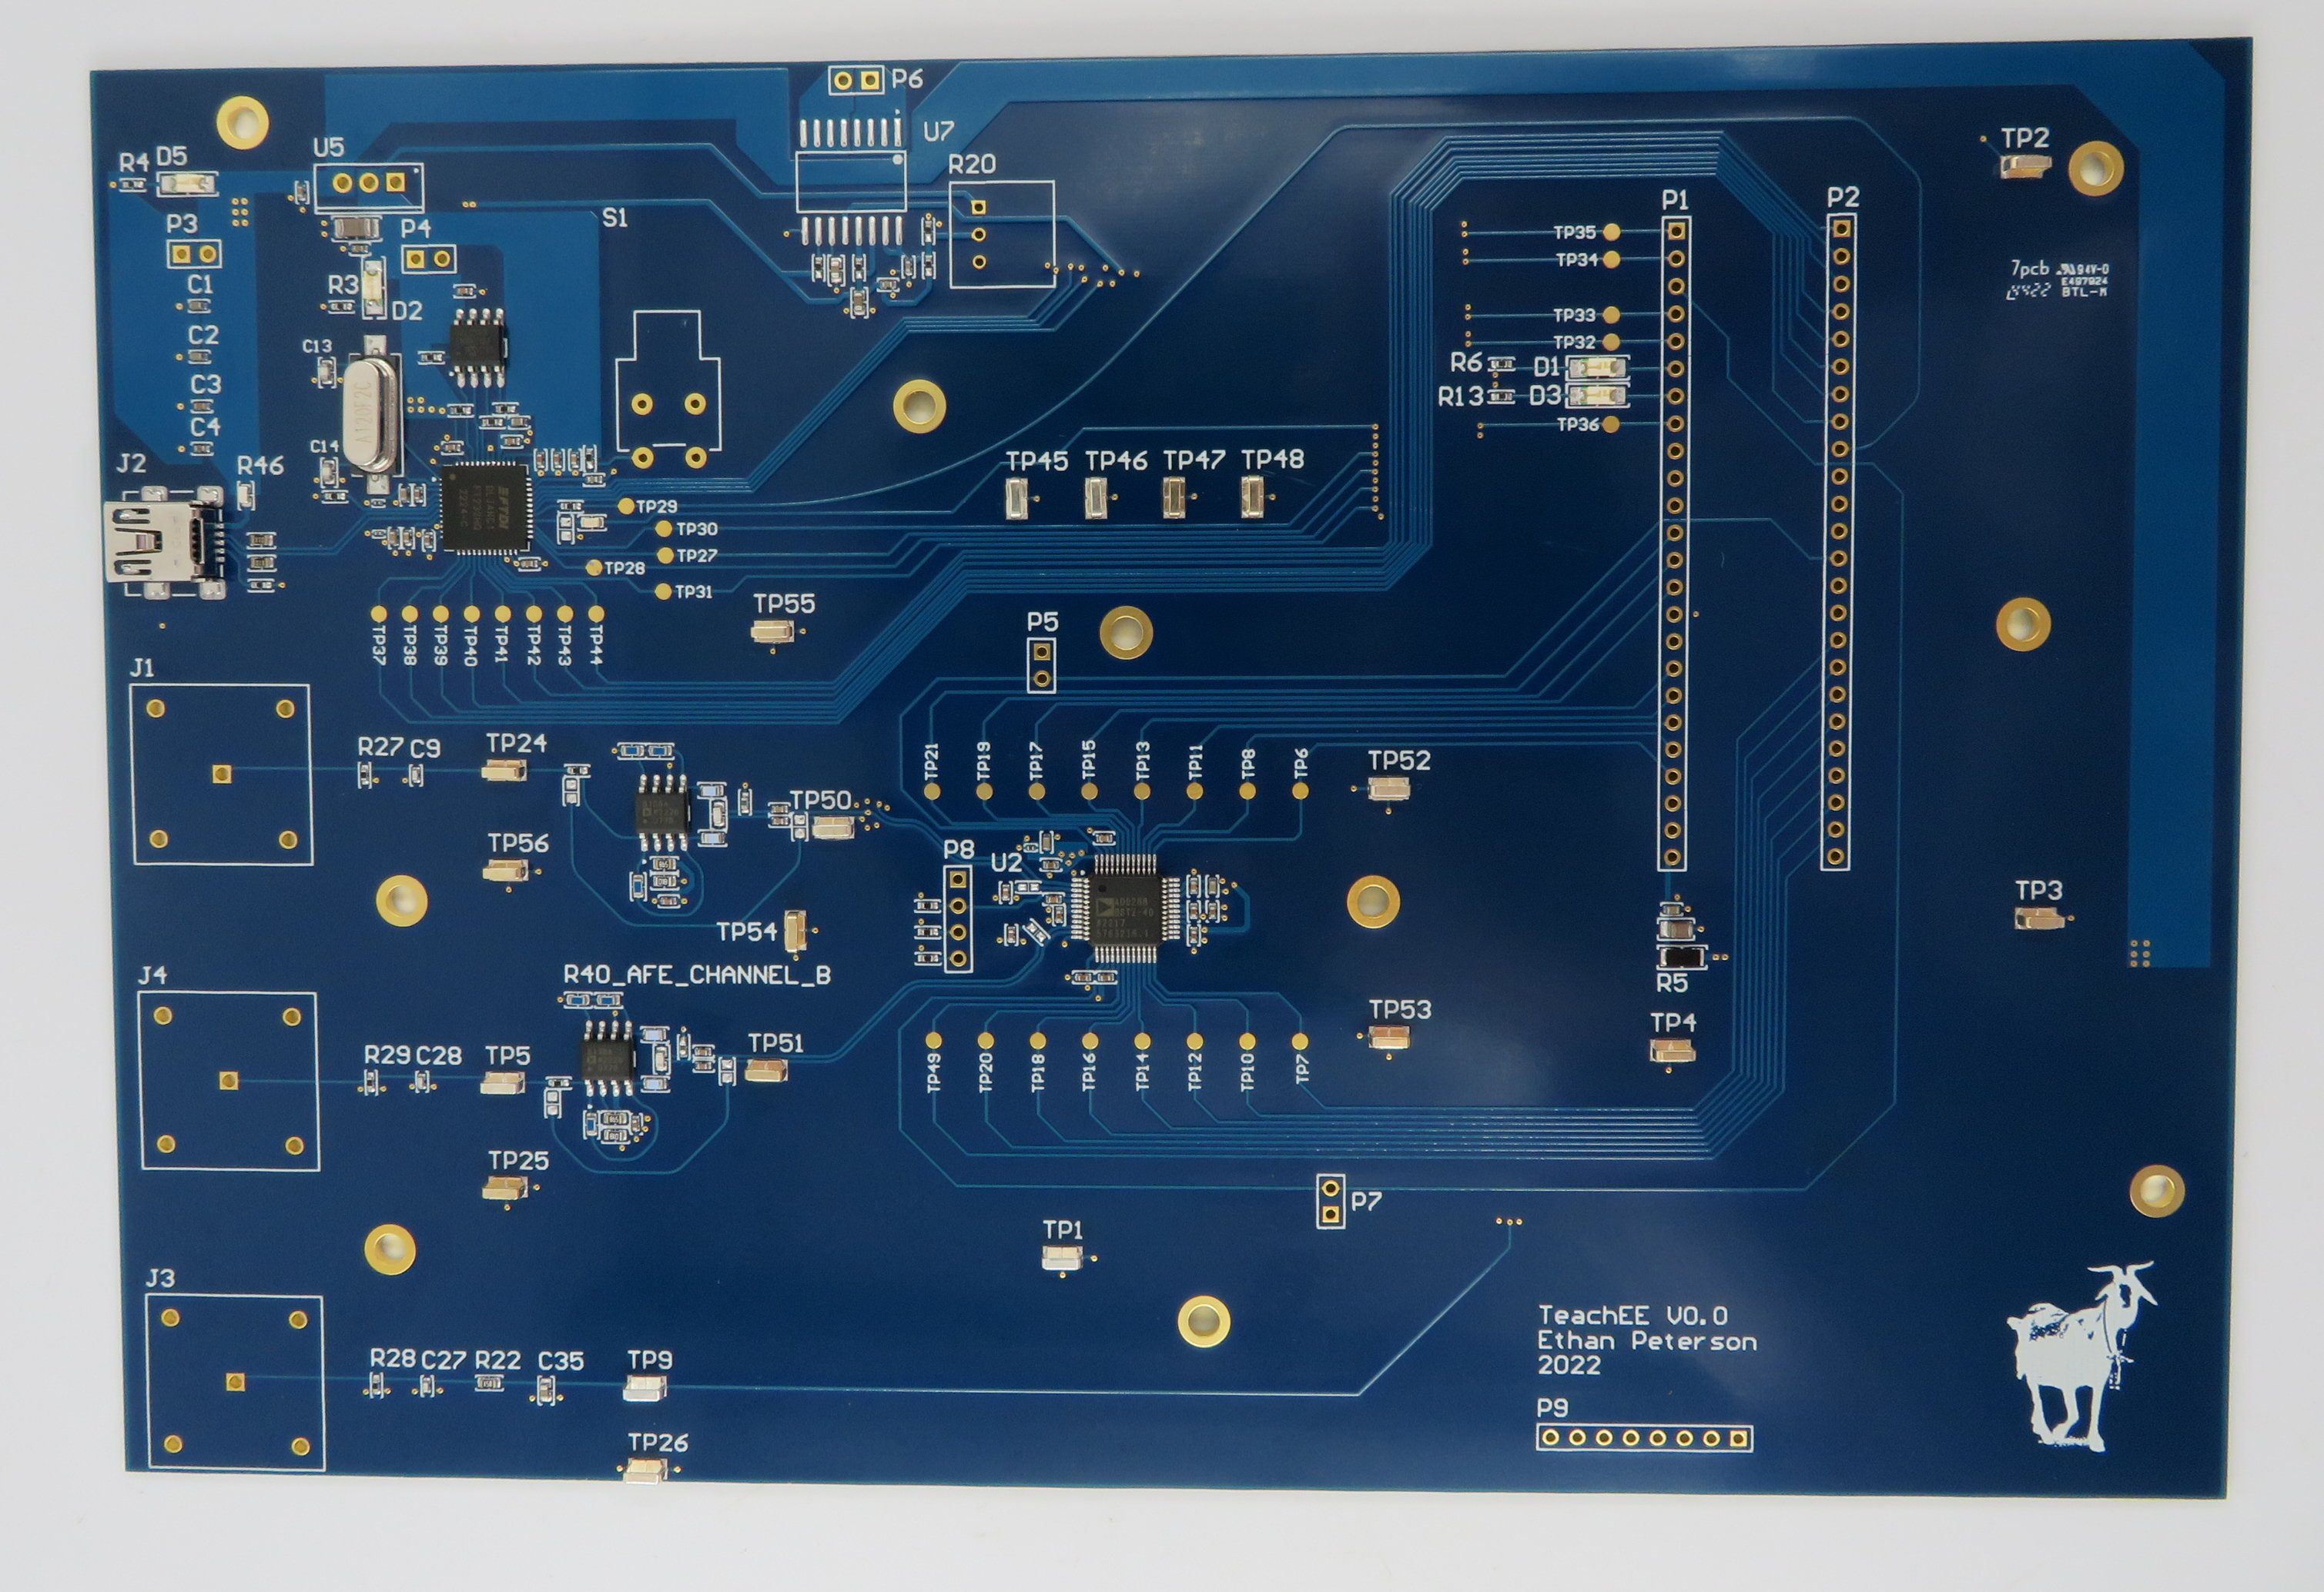
\includegraphics[width=\textwidth]{figures/pcb-front.JPG}
  \caption{PCB Front Side After Delivery}
  \label{fig:pcb-front}
\end{figure}

\begin{figure}[H]
  \centering
  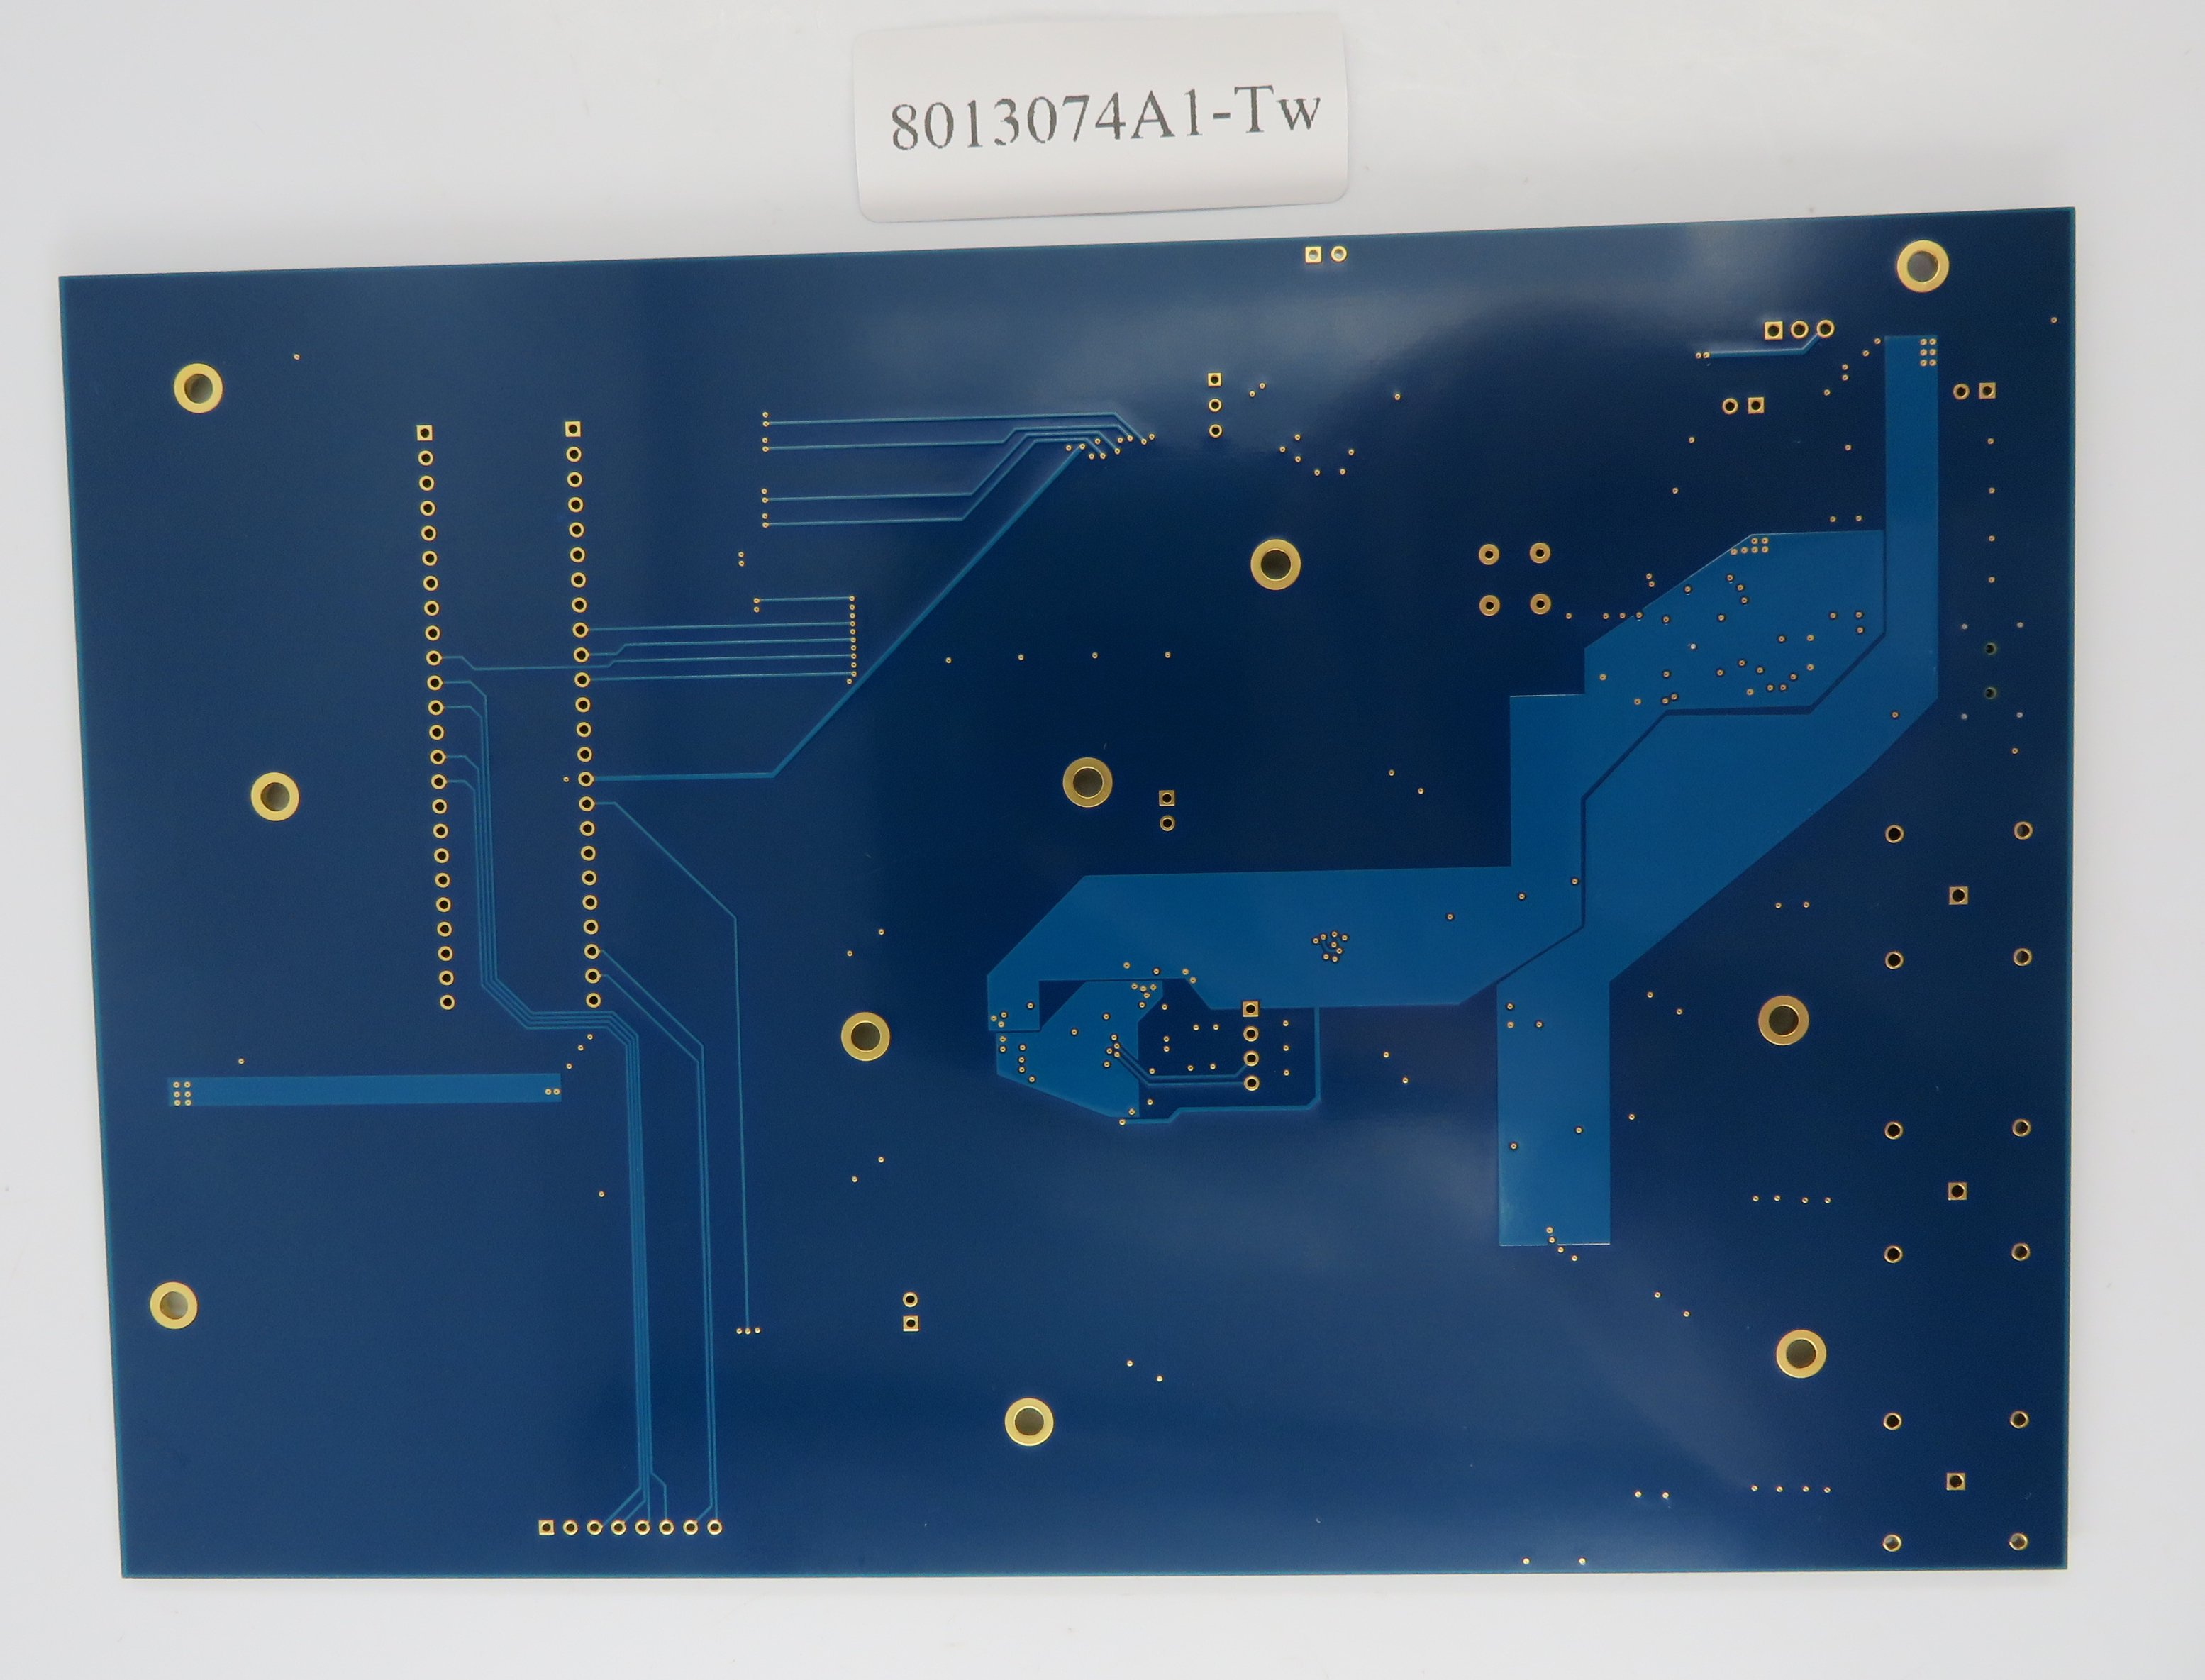
\includegraphics[width=12cm]{figures/pcb-back.JPG}
  \caption{PCB Back Side After Delivery}
  \label{fig:pcb-back}
\end{figure}

\begin{figure}[H]
  \centering
  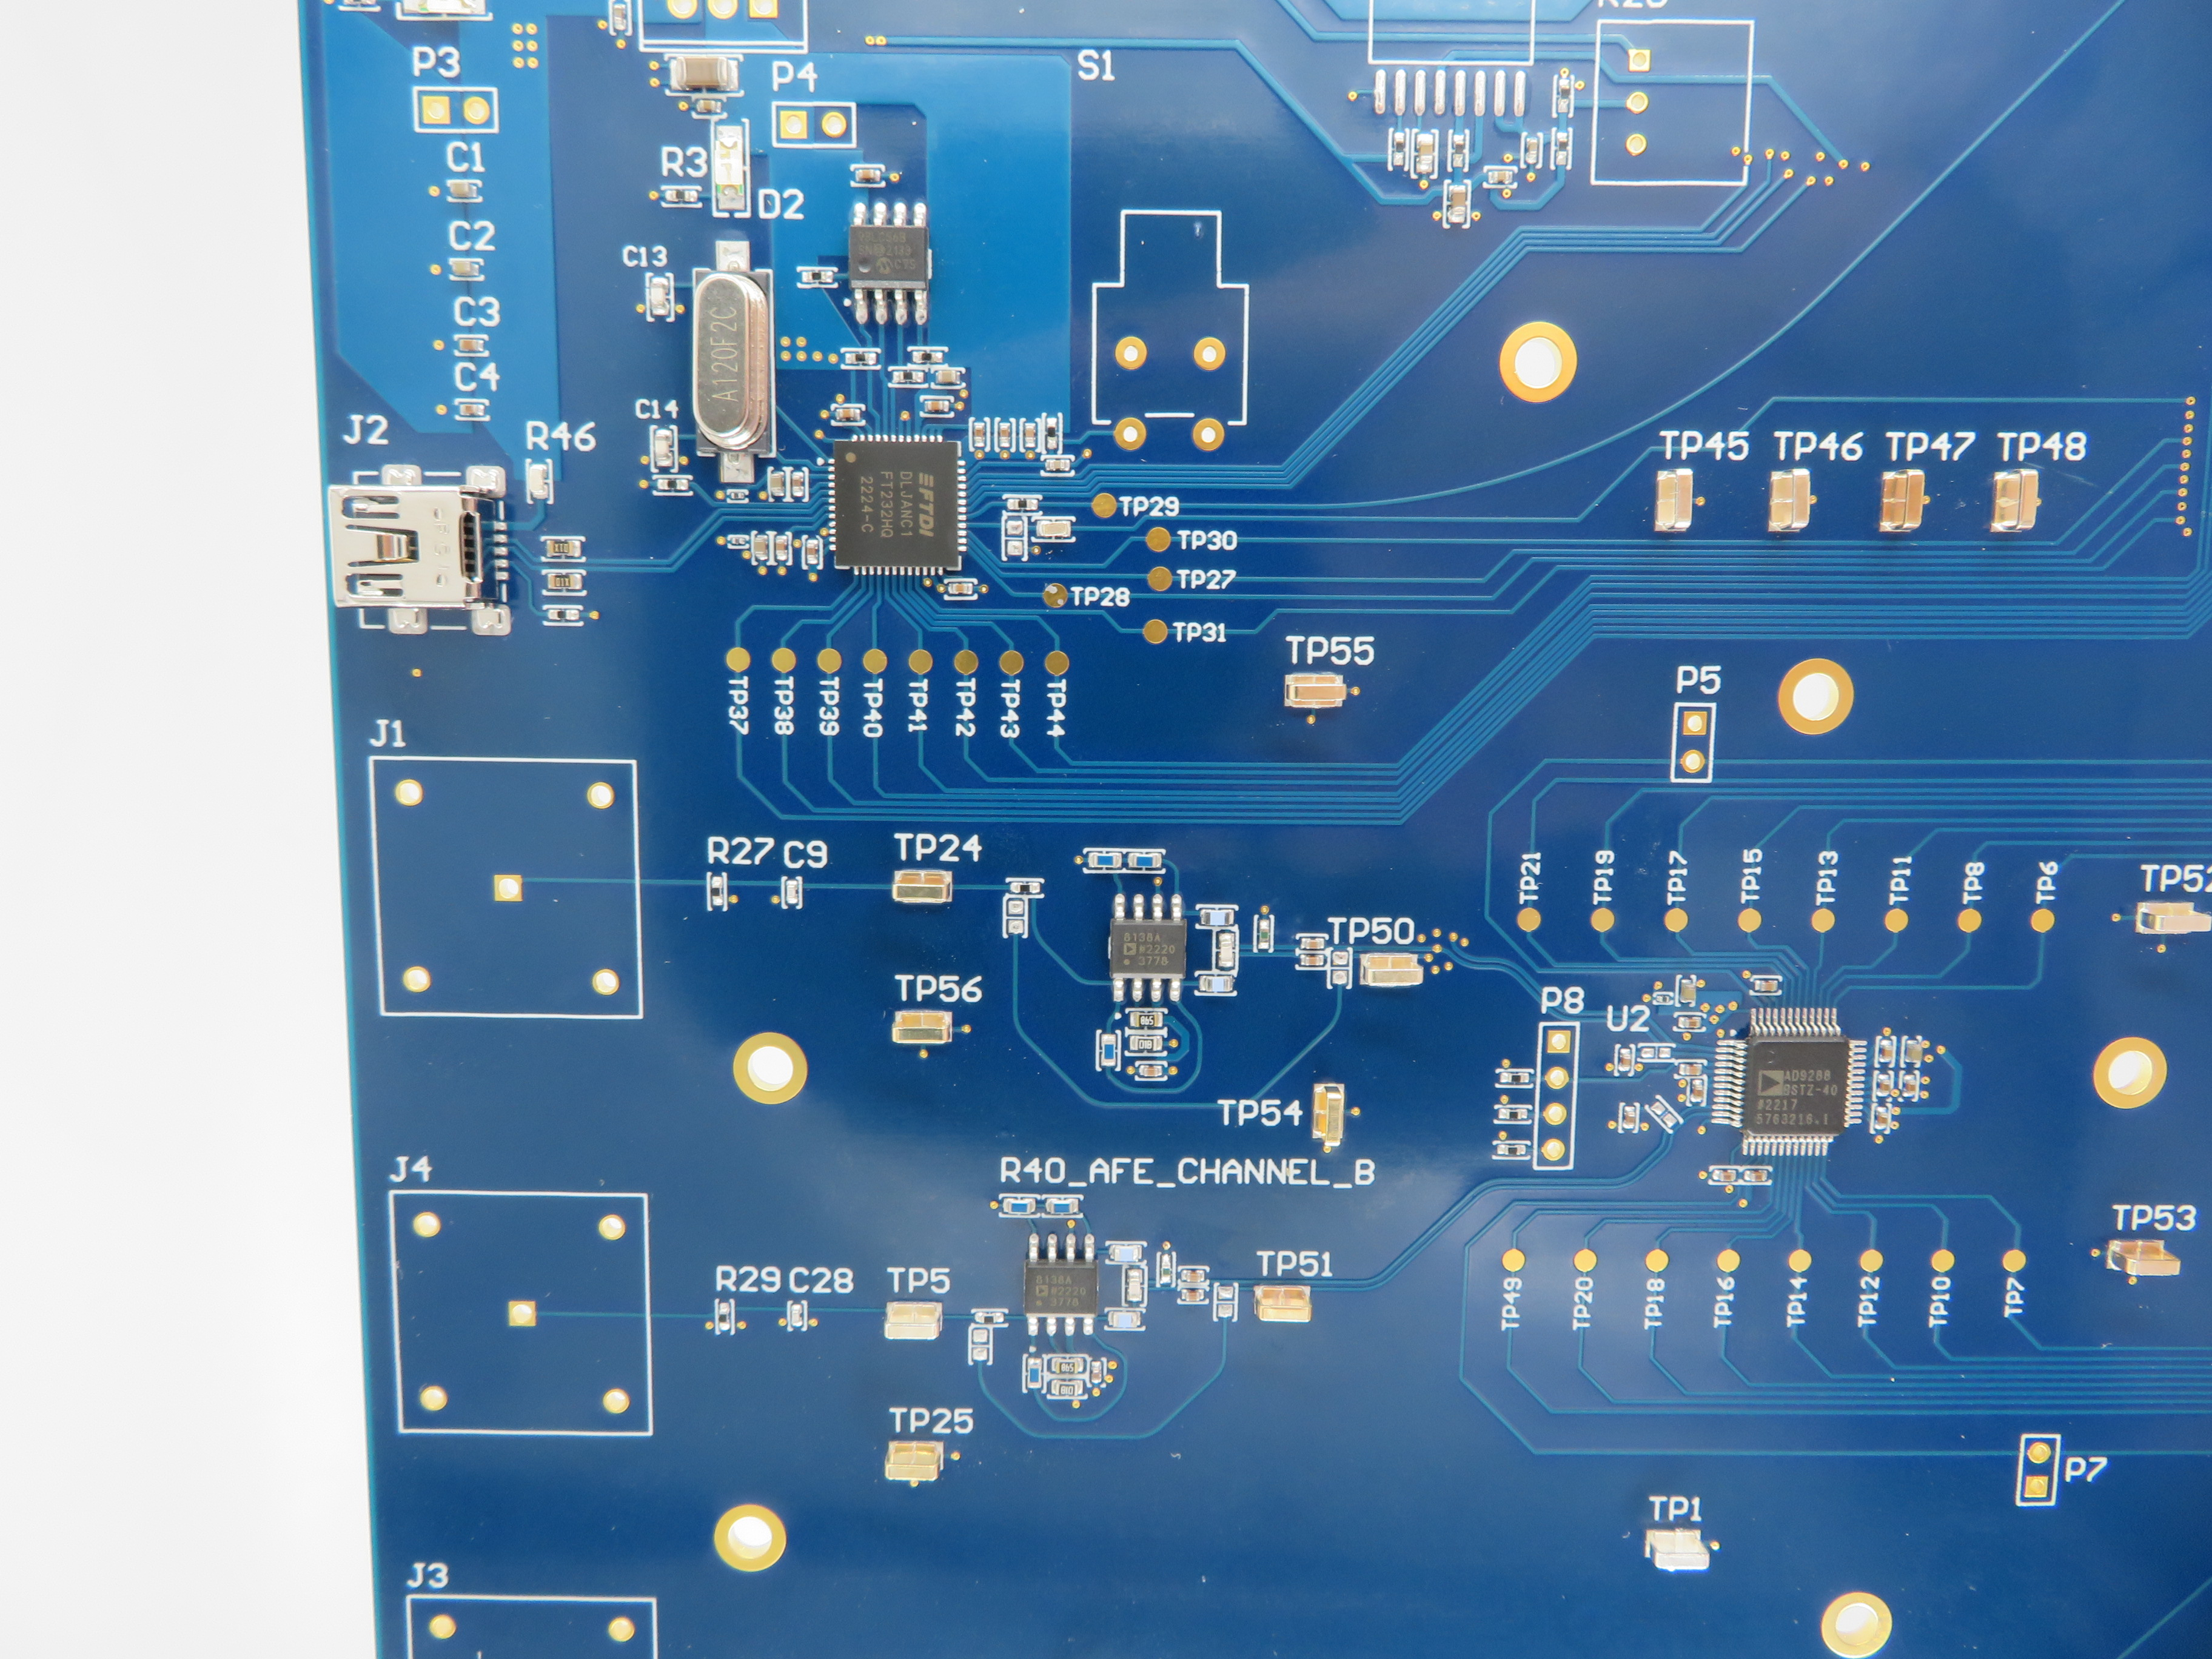
\includegraphics[width=12cm]{figures/pcb-closeup.JPG}
  \caption{Close up of the FIFO on the PCB}
  \label{fig:area-around-fifo}
\end{figure}

\subsubsection{Functional Testing}
All three assembled PCBs passed these inspection checks. Next, functional
testing was done on the three units. The functional tests are as follows.

\begin{enumerate}
  \item Plug TeachEE to a computer via the USB Mini connector. Open the FTDI
    Utility to check if the USB FIFO is detected. Ensure that the EEPROM can be
    read and that the USB device descriptor can be changed to \code{TeachEE}.
    After making the EEPROM change, unplug the device and plug back in. Check
    that the USB device is detected with the right descriptor information. This
    descriptor is used by the desktop software to identify the USB device as the
    oscilloscope.
  \item Use the \code{reader.py} script found in Appendix
    \ref{appendix:python-reader} to set the FT232HQ on TeachEE to synchronous
    data transmission mode 40.
  \item After setting the device to synchronous mode, connect an oscilloscope to
    the FT232HQ clock test point on the PCB. Verify that a \SI{60}{\mega\hertz}
    clock is supplied to the FPGA. The waveform should be a triangle wave. A
    screen capture of the clock waveform is given in Figure \ref{fig:ftdi-clk}.
    The triangle wave is not ideal but the FPGA locks to it successfully
    nonetheless.

  % \item Check the output voltage of the hall effect current sensor by probing
  %   the \code{VIOUT} pin with a DMM. This voltage should be approximately
  %   \SI{1.7}{\volt}, which represents a reading of \SI{0}{\ampere}.
\end{enumerate}

% TODO: add figure of the FTDI232HQ clock output
\begin{figure}[H]
  \centering
  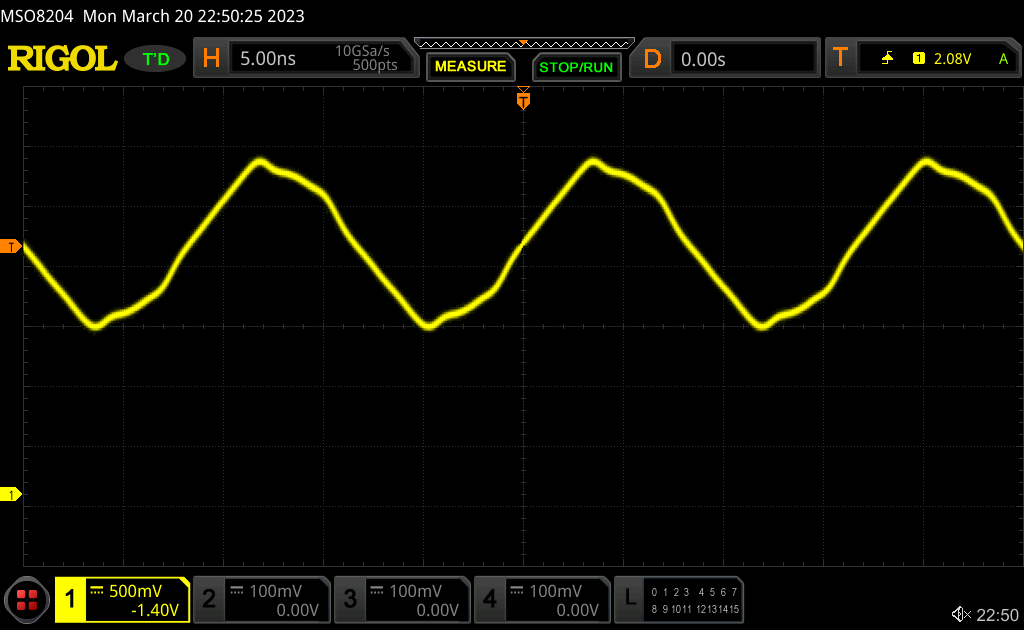
\includegraphics[width=12cm]{figures/ftdi-clk-cap.png}
  \caption{FT232HQ Clock Output Waveform}
  \label{fig:ftdi-clk}
\end{figure}

% write a little blurb about doing final assembly
All three PCBs passed the functional tests enumerated above. At this point, all
parts omitted from the assembly process were soldered onto the PCB. This included
all through-hole components on the board except for the voltage regulator, which
was soldered earlier for the power-up test. Through-hole parts were omitted
from the assembly order to keep costs low. Moreover, due to the chip shortage,
the hall effect current sensor had to be purchased separately and soldered
manually. The through-hole parts that were soldered manually included all the pin
headers for the FPGA, BNC connectors for the oscilloscope probes, and
through-hole test points. To protect the PCB from any conductive surfaces or ESD,
M3 standoff screws were installed into all the mounting holes. After this
final assembly step, the PCB was ready for software and FPGA development. The
FPGA module can be installed into the pin header and flashed. A fully assembled
TeachEE is shown in Figure
\ref{fig:pcb-final}.

\begin{figure}[H]
  \centering
  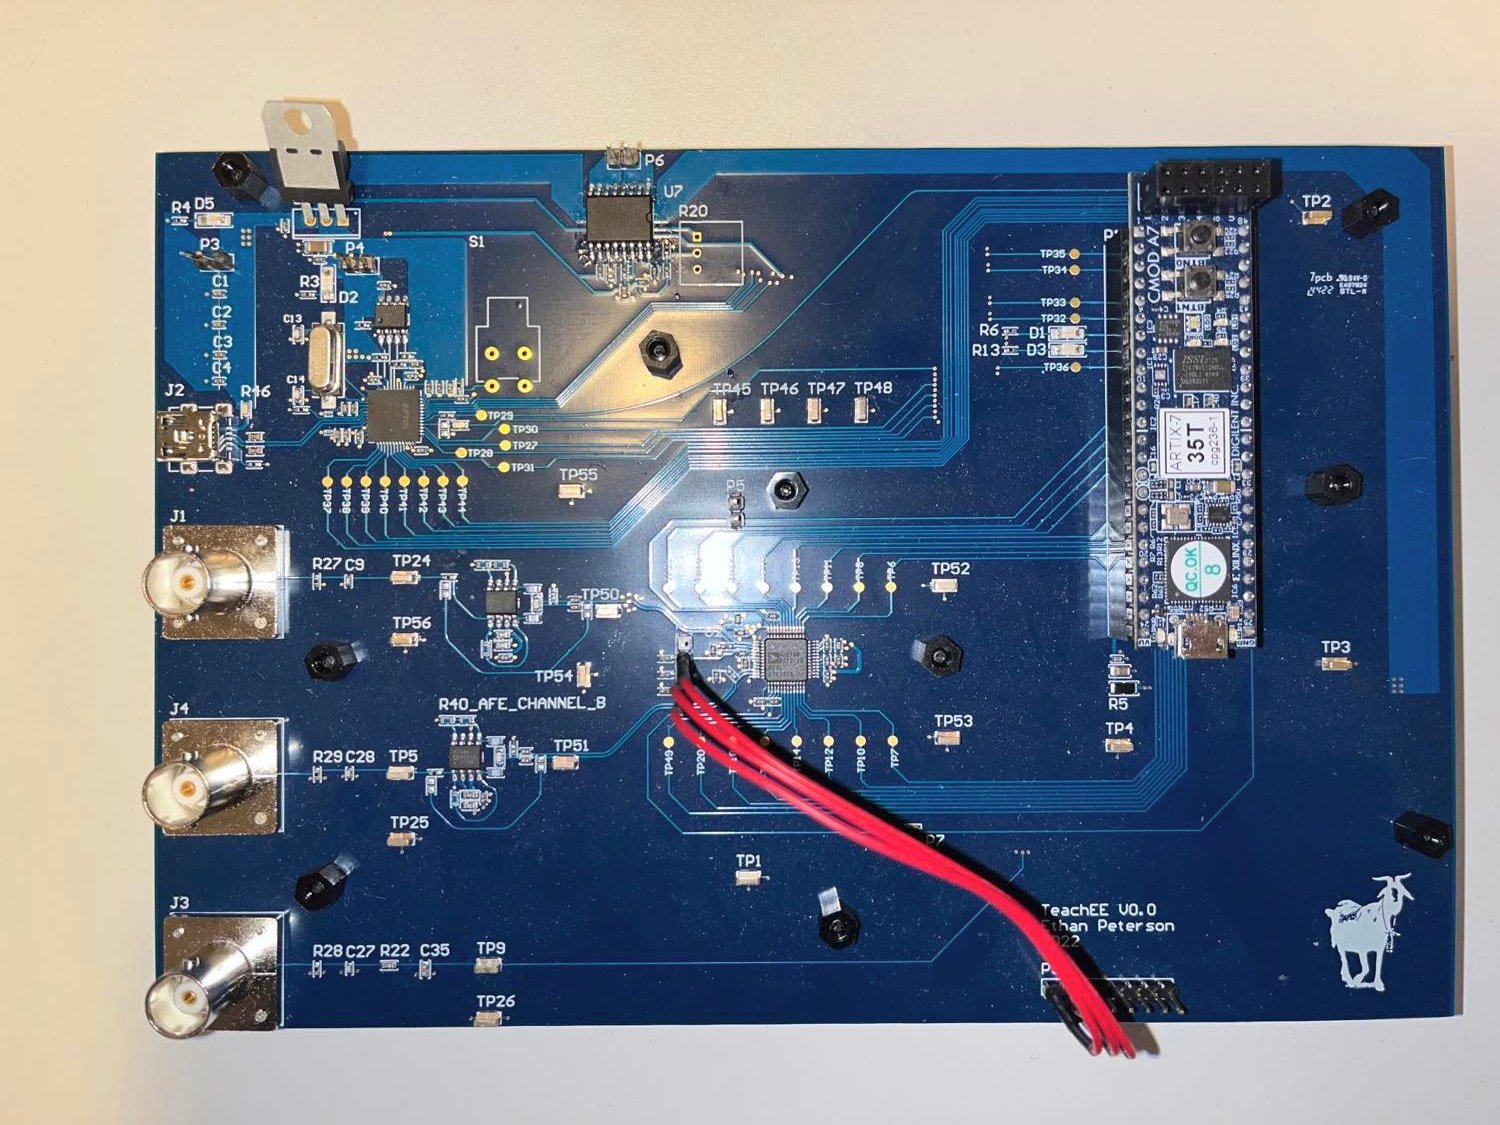
\includegraphics[width=\textwidth]{figures/pcb-final.jpg}
  \caption{Final Assembled TeachEE}
  \label{fig:pcb-final}
\end{figure}

\subsection{FPGA Verification} % ETHAN

% Talk about FPGA automated sims, testbenches CI ETC

FPGA code testing was a continuous process taking place throughout the
development cycle. SystemVerilog modules are tested and verified using
``testbenches''. Testbenches are modules that wrap around the module to be
tested and modulate the input signals through a variety of test cases
designed by the programmer. Example testbenches can be found in Appendix
\ref{appendix:rtl-leg-tb} and \ref{appendix:rtl-vunit-tb} respectively.

The verification of the code takes place on a per-module basis using one
testbench per module. This includes complex modules such as the packetizer, but
also simple modules that wrap AXIS interfaces. This allows each module to be
evaluated and verified independently of one another, ensuring easy integration
into the broader TeachEE codebase.

Initially, testbenches were made up of a finite state machine that applied
different inputs to the module, with the outputs being manually inspected by the
developer in ModelSim. These initial testbenches are shown in
Appendix \ref{appendix:rtl-leg-tb}. As the FPGA development process continued,
it quickly became difficult to manually inspect simulation waveforms due to the
large number of outputs and multi-cycle operations. An example of
one of the larger waveforms that needed to be manually inspected is shown in
Figure \ref{fig:xadc-packetizer-modelsim}.

\begin{figure}[H]
  \centering
  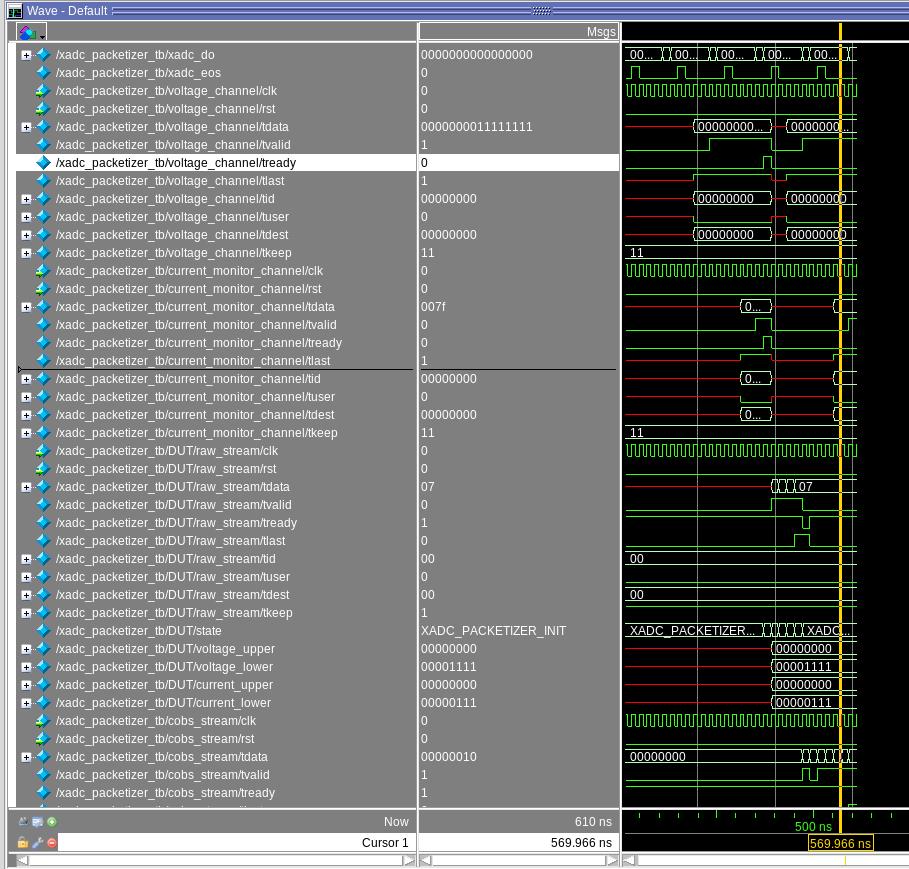
\includegraphics[width=\textwidth]{figures/modelsim-packetizer.png}
  \caption{Example ModelSim Waveform from a Packetizer Module}
  \label{fig:xadc-packetizer-modelsim}
\end{figure}

\subsubsection{Verification Automation With VUnit}
To speed up testbench development and debugging, an automated testing
framework, VUnit, was introduced. VUnit provides macros within SystemVerilog
to make assertions on the values of registers and wires \cite{vunit}. An example of
a SystemVerilog testbench written for use with VUnit is given in Appendix
\ref{appendix:rtl-vunit-tb}. This greatly improved development speed as checks
were automated and manual inspection was no longer required, except for specific
debugging tasks. Moreover, VUnit also allows testbenches to be specified in a
Python script. These Python scripts specify the dependencies and source files
needed to run the test as well. To run a testbench, it is as simple as running
the corresponding Python script so long as the simulation tool (ModelSim) and
VUnit package is installed. Each VUnit testbench has an accompanying Python file. A
Python testbench example is provided in Appendix \ref{appendix:python-vunit-tb}.

Another significant benefit of using VUnit is that it makes the testbenches
easily callable from a command line interface (CLI). In order to further
automate the testing, Continuous Integration (CI) was added to the TeachEE code
repository. The TeachEE code is hosted in a GitHub repository
\cite{teachee-github}. GitHub provides a tool called Actions which can be used
to run automated scripts on new code changes introduced to the repository in
pull requests \cite{github-actions-doc}. Since the VUnit testbenches are easily
callable from a script, a GitHub Actions script was introduced to run all the
testbenches on each pull request. The full source code is provided in Appendix
\ref{appendix:github-action-script}. The script installs ModelSim and Vunit, then
runs the testbenches, reporting any errors automatically when new code is pushed.
This ensured that new code did not break compatibility with older modules.

\subsubsection{Hardware Simulation with BFMs}
In many cases, additional supporting modules were needed to test a specific
module. Examples of this are the \code{ft232h}, \code{xadc_drp_axis_adapter},
and \code{hsadc_axis_adapter}. Since all of these modules were designed to
interact with the interface of a physical component on the PCB, mock interfaces
were needed to test the module. These device mocks are called
``Board Functional Models'' or BFMs. Each BFM is designed to respond in the same
way to input as the actual device itself. Of course, the BFM has no real data to
return so the data coming back will often be a preset value or known pattern.
The BFMs are written as finite state machines built to emulate the timing
diagrams provided by the manufacturer for a specific part. Usually, they are
more limited in their scope compared to the full device interface to limit the
potential for bugs. For example, \code{ft232h_bfm} only implements the write
interface of the FT232HQ as the USB reads are not used in TeachEE. The main
problem with BFMs is that they can produce bugs of their own. However, if the
BFM is correct, then a module interacting with the hardware modeled by the BFM
should work exactly as expected on the physical PCB. An example BFM that mocks
the interface of the XADC is given in Appendix \ref{xadc-bfm}.

\subsubsection{FPGA Bugs and Solutions} \label{sec:fpga-bugs}
During the FPGA and hardware verification process, the most difficult bugs were
at the intersection of the PCB hardware and FPGA. Specifically, bringing up the
FT232HQ and transmitting data proved difficult. The main reason for this is
that without the USB FIFO up and running, there is little visibility into the
FPGA firmware beyond the on-status LEDs and JTAG debugger. As a result, it was
extraordinarily difficult to distinguish whether an issue was hardware or FPGA
related. Eventually, it was discovered that an error in the state machine caused
the \code{ft232h} module to start sending data before the chip was ready to
accept it, leading to lost bytes or no bytes at all. After resolving this
misunderstanding of the device interface, it was discovered that the data was
being received but bytes were still missing. After probing the test points on the
USB FIFO using an external oscilloscope, it was discovered that data is sent for
one extra cycle after the USB FIFO stops accepting data, leading to dropped
bytes. This was not a misunderstanding of the device function, but rather a
misuse of asynchronous assignments in the code.

After resolving the dropped bytes and building a reliable channel, testing the
remaining modules in hardware was far simpler as the output of such modules
could be fed directly to the connected computer and evaluated.

Aside from Data Integrity, power-on race conditions proved an issue for the
FPGA design. Since the design is dependent on an external clock generated by the
USB FIFO, the data transmission often did not start up
correctly if the clock was not received in a timely manner during the boot
sequence. The clock was not available immediately since the device first had be
set to synchronous mode by the software to produce the clock. This issue was
resolved by probing the clock output pin of the FT232HQ during start-up and
triggering on the first clock edge. Once the source of the problem was
established, a clever use of the \code{locked} output of the PLL was used to hold
all modules in reset until the clock becomes available.

\subsection{Software Verification} \label{sec:software-verification} % ERIC
% Rust CI, Testing with mock byte streams? 
% Threading model iteration, trigger iteration
% Testing decoding algo with recorded bytestream and asserts (adding error handling)
% FFT testing (using lab sig gen, discovered incorrect sample rate)
Overall software validation was done throughout the development life cycle using
two tools. The first tool was a mock bytestream generator that populates the channel
buffers with sawtooth waves. The generator simulates data arriving from the hardware
and allowed developers to test Controller and App functionality without TeachEE
hardware. This greatly increased development flexibility as the developers could
write code and immediately test it remotely. For example, the trigger functionality
correctness was verified with these mock bytestreams rather than the hardware. The mock
bytestream code is provided in Appendix \ref{appendix:software-sine}. The
second tool was an automated GitHub Action script run on every branch that builds the
software, checks code formatting, and runs a linter to catch common mistakes. This
tool ensured that code merged to the main branch was written with good style and did
not introduce any build errors. This script is provided in Appendix
\ref{appendix:software-script}.

\subsubsection{Design Iteration} \label{sec:soft-performance-issues}
Severe performance issues were encountered while implementing the initial
software design described in Section \ref{sec:soft-design}. The frame rate of the
UI was limited to approximately ten frames per second. This issue was caused by high
levels of mutex contention: the USB Manager thread would repeatedly acquire the
mutex, thereby starving the App thread.
Because threads did not take turns, they could overwrite new data or read stale
data. The new implementation addressed these concerns by using monitors to
prevent redundant read/writes and limit contention, and runs at an average of fifty
frames per second. These frame rates were measured using instrumentation code run
in the UI update function. The code is provided below.

\setstretch{1}
\begin{minted}{rust}
  ...
  self.counter += 1;
  if self.start.elapsed() > Duration::from_secs(1) {
      println!("{}", self.counter);
      self.counter = 0;
      self.start = Instant::now();
  }
  ...
\end{minted}
\setstretch{2}

The triggering functionality also underwent design iteration. The initial
triggering algorithm used a moving average sliding window as the noise
mitigation strategy. It required that the average of the last \code{WINDOW_SIZE}
samples be less than the currently analyzed sample, in addition to requiring that the
currently analyzed sample be greater than the trigger threshold. The sliding window
iterator is shown below.

\setstretch{1}
\begin{minted}{rust}
  const WINDOW_SIZE: usize = 10;
  let mut sum: f64 = src[lower_idx..(lower_idx + WINDOW_SIZE)].iter().sum();
  // Iterate over all windows of size WINDOW_SIZE + 1. The first WINDOW_SIZE
  // samples are used to calculate the average value of previous samples,
  // which is then compared to the last sample. This is done to find a
  // rising edge while attempting to filter out noise.
  let first_higher = src[lower_idx..]
      .windows(WINDOW_SIZE + 1)
      .position(|window| {
          let val = *window.last().unwrap();
          val >= trigger && sum / (WINDOW_SIZE as f64) < val || {
              // Update sliding window.
              sum += val;
              sum -= *window.first().unwrap();
              false
          }
      });
\end{minted}
\setstretch{2}

Although this algorithm functioned well, it produced slightly unstable
waveforms and did not consistently trigger at the exact same position on every
iteration of a signal. Furthermore, concerns were made about the validity of
the algorithm and the team wanted a more conventional implementation. These issues
led to the research and implementation of the current hysteresis-based triggering
algorithm described in Section \ref{sec:soft-controller}.

\subsubsection{Feature Testing}
Every implemented feature was rigorously tested before proceeding with new features.
For example, the packet decoding functionality was tested using bytestreams
redirected from the hardware to a file. Because the voltage and current values
from the file were known, they could be compared to the voltage and current values
after being decoded by the software algorithm. This verified that the packets
were being decoded correctly and that the bytes were mapped to the right
voltage/current values. Additionally, assertions were used to alert the team
of any unexpected packet errors. These assertions led to the discovery of the
packet encoding problem described in Section \ref{sec:fpga-bugs}. They also
prompted additional decoder error handling as the bytestream channel was found
to not be completely reliable.

Software bugs were also discovered during testing of the frequency spectrum
analysis feature. The library provided spectrum analysis function produced
frequencies twice that of signals generated using a lab signal generator.
This factor-of-two error was ultimately determined to be caused by an
incorrect sample rate assumption in software. Although the hardware was
indeed sampling at \SI{1}{\mega\samplepersec}, the sample rate per channel
with two channels was actually \SI{500}{\kilo\samplepersec}. This correction
fixed both the FFT functionality and the plots' time scales.

\section{Project Planning and Budgeting} % ERIC

The following table lists the original milestones associated with this project.
\begin{table}[H]
    \caption{Milestones}
    \begin{tabularx}{\textwidth}{l|l|l|l}
        No. & Milestone & Due date & Responsible Member(s) \\
        \hline
        1 & Design and order PCB & Week 4 & Ethan \\
        2 & Create skeleton of application & Week 11 & Tim \\
        3 & Submit blueprint report & Week 11 & All members \\
        4 & Verify PCB is functional & Week 12 & Ethan \\
        5 & Read values from USB driver & Week 13 & Tim and John \\
        6 & Create basic UI and waveform display & Week 14 & Eric \\
        7 & FPGA programming & Week 16 & Ethan \\
        8 & Implement oscilloscope triggering & Week 16 & John \\
        9 & Implement CSV exporting and all UI functionality & Week 17 & Eric \\
        10 & Testing of application & Week 18 & Tim, Eric, and John \\
        11 & Testing of PCB & Week 18 & Ethan \\
        12 & Testing of complete system & Week 20 & All members \\
        13 & Open House & Week 22 & \\
        14 & Final deliverable & Week 23 & \\
        15 & Final project report & Week 24 & All members
    \end{tabularx} 
\label{hw:milestones-table}
\end{table}

Many milestones were completed earlier than planned; in particular, the full FPGA
and UI work were completed between weeks 12 and 13, and basic triggering was
implemented in week 15. Due to the severe software performance issues described in
Section \ref{sec:soft-performance-issues}, developing a new design became the top priority.
This slightly delayed some less important UI work, but all required functionality was
completed by week 19. Furthermore, many stretch goals were achieved, including
reading from four concurrent channels, advanced triggering, and frequency spectrum
analysis. Also, minimal testing was required near the end of the timeline as most
issues were solved during development through iterative testing.

Table \ref{tab:abbreviated-bom} breaks down the cost of the PCB
fabrication and assembly as quoted by the supplier. The supplier contracted for
TeachEE is Bittele (7PCB). Bittele takes care of both the fabrication and
soldering of the PCBs. Moreover, Bittele takes the generated output from the EDA
software (Altium) and procures all the parts directly to their facility. The
procurement cost is expanded in the budget table with the major functional
components on the PCB. An exhaustive list is not included as there are hundreds
of miscellaneous resistors, capacitors, and inductors with marginal cost.

A full unit of the PCB cost \$80 less than the target budget. This left
additional budget to purchase replacement components and
cover unexpected expenses. Two additional backup boards were ordered in case the main
board failed. Fortunately, the team did not encounter any hardware failures during the
course of the project and therefore did not require any replacing of the board or its
components. The full BOM for the PCB is provided in Appendix \ref{appendix:bom}.

\begin{table}[H]
    \caption{TeachEE Bill of Materials}
    \begin{tabularx}{\textwidth}{l|l|l}
        \textbf{Item / Part Number} & \textbf{Supplier} & \textbf{Cost (CAD)} \\
        \hline
        PCB Fabrication & Bittele & \$104.37\\
        PCB Total BOM Procurement & Bittele & \$126.67\\
        \hline
        \textbf{Major Components (Included in cost above)}& &\\
        \hline
        AD9288BSTZ-40 ADC & Digi-Key & \$14.70\\
        AD8138ARZ-R7 ADC Driver & Digi-Key & \$26.85\\
        FT232HQ-REEL USB FIFO & Digi-Key & \$6.41\\
        ACS720KLATR-15AB-T Current Sensor & Digi-Key & \$9.81\\
        \hline
        PCB Assembly & Bittele & \$289.76\\
        \hline
        Total & & \$520.80\\
        \hline
        Budget Remaining & & \$79.20
    \end{tabularx} 
\label{tab:abbreviated-bom}
\end{table}

\section{Stakeholder Needs} \label{sec:stakeholder-needs} % John / Tim
%% Describe how you considered stakeholder needs in your design, and how factors
%% like safety, privacy, codes/standards, manufacturability, ethics and cost were
%% considered in your design.

% JOHN should use this section to discuss why our device is more suited to EE
% undergrads than what is currently on the market. Tim should provide some input
% on manufacturability and cost too.

% Add something about how an EE professor and stakeholder (Whitehall) noted that
% the scopes provided in his class's lab kits didn't have a good FFT implementation
% (difficult to tell whether the screen showed time domain or FFT, could not
% simultaneously display both time and frequency plots) so we took his needs into
% account with our implementation (which clearly shows time or FFT and both at the
% same time)

\subsubsection{Features and Quality}

%% Ethan, if you could elaborate on why the kits were bad that would be great.
%% John finds it difficult to comment since he did not use the kits
%% Emphasis on the "quality" point

%% and to double check, we did indeed have scroll to zoom functionality?

In the online electrical engineering labs during the pandemic, an electronics
professor noticed issues with the kits provided to students. There was a general
lack of quality and brittleness which caused students to require replacement
kits. Additionally, the implementation of certain features were poor; the
display was unable to simultaneously show the frequency and time domain, and it
was poorly indicated which was currently being displayed. 

Beyond the lab kits, the archaic design of a typical oscilloscope can be
improved upon. Rather than rotating physical knobs to adjust the display, it is
more intuitive to interact with the application like you would any other:
through the interface of a computer application. This benefits novice engineers
that are unfamiliar with traditional oscilloscopes' interfaces.

TeachEE addresses these stakeholder needs. The
application is intuitive to use, with the ability to click and drag to adjust
the waveform display, as well zooming via mouse scroll. It can also
intuitively display the spatial and time domain of signals at the same time.

\subsubsection{Safety}

As was mentioned in Section \ref{sec:software-verification}, the software has been
thoroughly tested to ensure stability for users. In particular, the choice of
Rust in the presence of complex threading models yields a high degree of
confidence that undefined behaviour is avoided. Given that TeachEE can export
CSV files onto the host computer, this opens a vector of damage. If these
precautions were not taken then there is the possibility that TeachEE enters an
invalid state and writes to the user's computer in an undesirable way.

A computer can be damaged through the USB port by devices such as ``USB Killers''
\cite{usb-killer}. Since TeachEE works with high voltage and current, it is
important to ensure protection of the user's computer during operation. The
computer is protected from backflow by diodes in the voltage regulator.
Additionally, on the device itself, the analog front end clamps voltages that
are too high.

\subsubsection{Manufacturing Cost}

The viability of manufacturing TeachEE at scale is promising due to the current
design's significant drop in unit cost at increased volume.  At scales greater
than 100 units, the team estimates that the cost-per-unit could drop as low as \$250. This
reduction in cost provides an opportunity for competitive pricing compared to
the PicoScope\textregistered~4000, a USB oscilloscope with similar
specifications to TeachEE. The manufacturers' price for a
PicoScope\textregistered~4000 starts at \$930, indicating a potential profit of
up to 272\% if the TeachEE were sold at scale for \$930 per unit
\cite{picoscope}. These figures suggest that TeachEE could be a viable product with
the potential for a good return on investment.

\section{Compliance with System Requirements} % John
%% Compliance with specifications – Include your original specifications table from
%% the Blueprint and add extra column to it as shown below and report what you
%% obtained with your final design. If any of your specs were not achieved or fell
%% outside the tolerance values, explain why in this section. Your mark for this
%% section depends on how close you got to your specs

% NOTE: John please finish off this section, i just did the tables, - ethan
The following tables outline the target hardware and software specifications of
this project. The hardware and software specification evaluations are given in
Tables \ref{tab:hw-spec-eval} and \ref{tab:sw-spec-eval} below, and show that
the prototype meets or exceeds the specifications in all areas.

\begin{table}[H]
    \caption{Hardware Specification Evaluation}
    \begin{tabularx}{\textwidth}{c|c|c|p{5cm}}
        Specification & Target Value & Achieved? & Comments \\
        \hline
      Voltage Input Bandwidth&\SI{100}{\kilo\hertz}& Yes & Ultimately \SI{500}{\kilo\hertz} of bandwidth was achieved through the low speed ADC and \SI{20}{\mega\hertz} through the high speed ADC.\\
        \hline
        Current Input Bandwidth&\SI{100}{\kilo\hertz}& Yes & This bandwidth matches the hall effect sensor.\\
        \hline 
        Measurable Current Range&\SI{-15}{\ampere} to \SI{+15}{\ampere}& Yes & Matches the specification of the sensor.\\
        \hline
        Measurable Voltage Range& \SI{0}{\volt} to \SI{3.3}{\volt} & Yes & This was achieved in both XADC and HSADC channels.\\
        \hline
        Number of Current Input Channels& $1$ & Yes & \\
        \hline
        Number of Voltage Input Channels& $1$ & Yes & Two additional voltage channels were added using the HSADC.\\
        \hline
        Power Input Voltage Rating& \SI{5}{\volt} & Yes & USB voltage is used as supply and the regulator is tolerant up to \SI{12}{\volt}.\\
        \hline
        Power Current Consumption Rating& \SI{500}{\milli\ampere} & Yes & Current draw has not exceeded \SI{500}{\milli\ampere} in any operation setting.\\
        \hline
        Voltage Sample Rate& \SI{1}{\mega\samplepersec} & Yes & The XADC can sample at \SI{1}{\mega\samplepersec} and HSADC can sample at \SI{40}{\mega\samplepersec}.\\
        \hline
        Current Sample Rate& \SI{1}{\mega\samplepersec} & Yes & \\
        \hline
        PCB Thickness& \SI{1.6}{\milli\metre} & Yes & Thickness was exactly 1.6 mm in a four-layer stackup. \\
        \hline
        PCB Dimensions& $\pm \SI{400}{\milli\metre\squared}$ & Yes & The tolerance given is less than the final size of the PCB.\\
        \hline
        Voltage Sample Error & $\pm \SI{20}{\percent}$ & Yes & Values match almost exactly to the Rigol scope in the Sci '65 lab through empirical testing.\\
        \hline
        Current Sample Error & $\pm \SI{20}{\percent}$ & Yes & Current readings match a DMM within this tolerance.\\
        \hline
    \end{tabularx} 
\label{tab:hw-spec-eval}
\end{table}

\begin{table}[H]
  \caption{Software Specification Evaluation}
  \begin{tabularx}{\textwidth}{p{8cm}|l|p{6cm}}
    Specification & Achieved? & Comments\\
    \hline
    The software shall be able to modify the horizontal and vertical scales of the plot. & Yes & Multiple plot navigation methods, including touch screen and trackpad compatibility. \\
    The software shall be able to modify the trigger voltage. & Yes & Triggering algorithm was exceptionally stable. \\
    The application shall be deployable to Windows, macOS, and Linux. & Yes & \\
    \hline
    The software shall be able to capture voltage samples and export them to a CSV file. & Yes & \\
    The software shall receive samples via the FTDI 232 in synchronous mode. & Yes & \\
    \hline
    The software shall be able to render waveforms at a rate of \SI{30}{\hertz} on screen. & Yes & Achieved \SI{50}{\hertz} with final design. \\
    \hline
  \end{tabularx} 
  \label{tab:sw-spec-eval}
\end{table}

\section{Conclusions \& Recommendations} % Tim
%% Conclusions and recommendations – provide commentary on the main technical
%% lessons learned from this project; is there potential for lasting impact for
%% this project beyond this course? Can more research be done in an area? Should
%% someone tackle this problem again but using a different approach? Is there
%% potential for commercialization? If this were to be scaled out to a commercial
%% version how would it be manufactured and what would the cost be? Speculate about
%% the market size for such a product. If the product makes it to the market, what
%% are the potential positive and adverse societal and cultural impacts of the
%% product? How can the adverse impacts be mitigated?
% See open house poster for inspiration

Developing TeachEE provided the team with several valuable technical lessons,
including the value of using Rust for applications requiring high performance
and concurrency. Rust's focus on memory safety and zero-cost abstractions makes
it an ideal choice for building high-performance systems with low-level
control. The team found that Rust enabled them to write code that was both safe
and efficient, allowing them to achieve the necessary performance requirements
for the TeachEE prototype. Overall, the team believes that Rust was a key
factor in the success of the TeachEE project, and they plan to continue using
it for future projects that require high performance and concurrency.

Another key lesson learned is to avoid assuming ideal specifications for hardware
components, for example, assuming ideal speeds for USB 2, which were not
achievable in practice. Such assumptions led to unexpected issues in the
prototype. As a result, adjustments needed to be made to accommodate the actual
capabilities of the components. This experience taught the team the importance
of conducting thorough research on the specifications of hardware components
and testing them under realistic conditions.

In conclusion, the team considers the TeachEE prototype to be a success
and are proud to have met or exceeded all the product requirements.
If TeachEE were to be launched as a product, it could 
potentially create lasting impact on the field of engineering by reducing the
barrier of entry for aspiring electrical engineers. TeachEE's low cost makes it
more accessible to students and hobbyists who may not have access to expensive
laboratory equipment (see Section \ref{sec:stakeholder-needs}). By providing an
affordable tool for learning and experimentation, TeachEE can help to
democratize access to electrical engineering education and enable a more diverse
range of individuals to engage with the discipline. For these reasons, the team
believes further development in products like TeachEE is worthwhile.

\section{Overall Team Effort}
The following table quantifies the percentage effort each team member expended
on all aspects of the project.

% NOTE: I think we will need to add some further reflection here about how the
% project went overall, it is in the rubric
\begin{table}[H]
  \caption{Team Effort Table}
  \centering
  \begin{tabularx}{10cm}{l|l}
    \textbf{Name} & \textbf{Effort Expended \%}\\
    \hline
    Ethan Peterson & TODO \\
    \hline
    Eric Yang & TODO \\
    \hline
    Timothy Morland & TODO \\
    \hline
    John Giorshev & TODO \\
  \end{tabularx} 
\end{table}
\newpage

\setstretch{1.4}
\bibliographystyle{IEEEtran}
\bibliography{report}

\newpage
\setstretch{1}
\newcommand{\changelocaltocdepth}[1]{%
  \addtocontents{toc}{\protect\setcounter{tocdepth}{#1}}%
  \setcounter{tocdepth}{#1}%
}
\changelocaltocdepth{1}

\pagestyle{empty}

    \begin{appendices}
        \begin{landscape}
        \section{Schematics}
        \label{appendix:schematic}
    \centering
    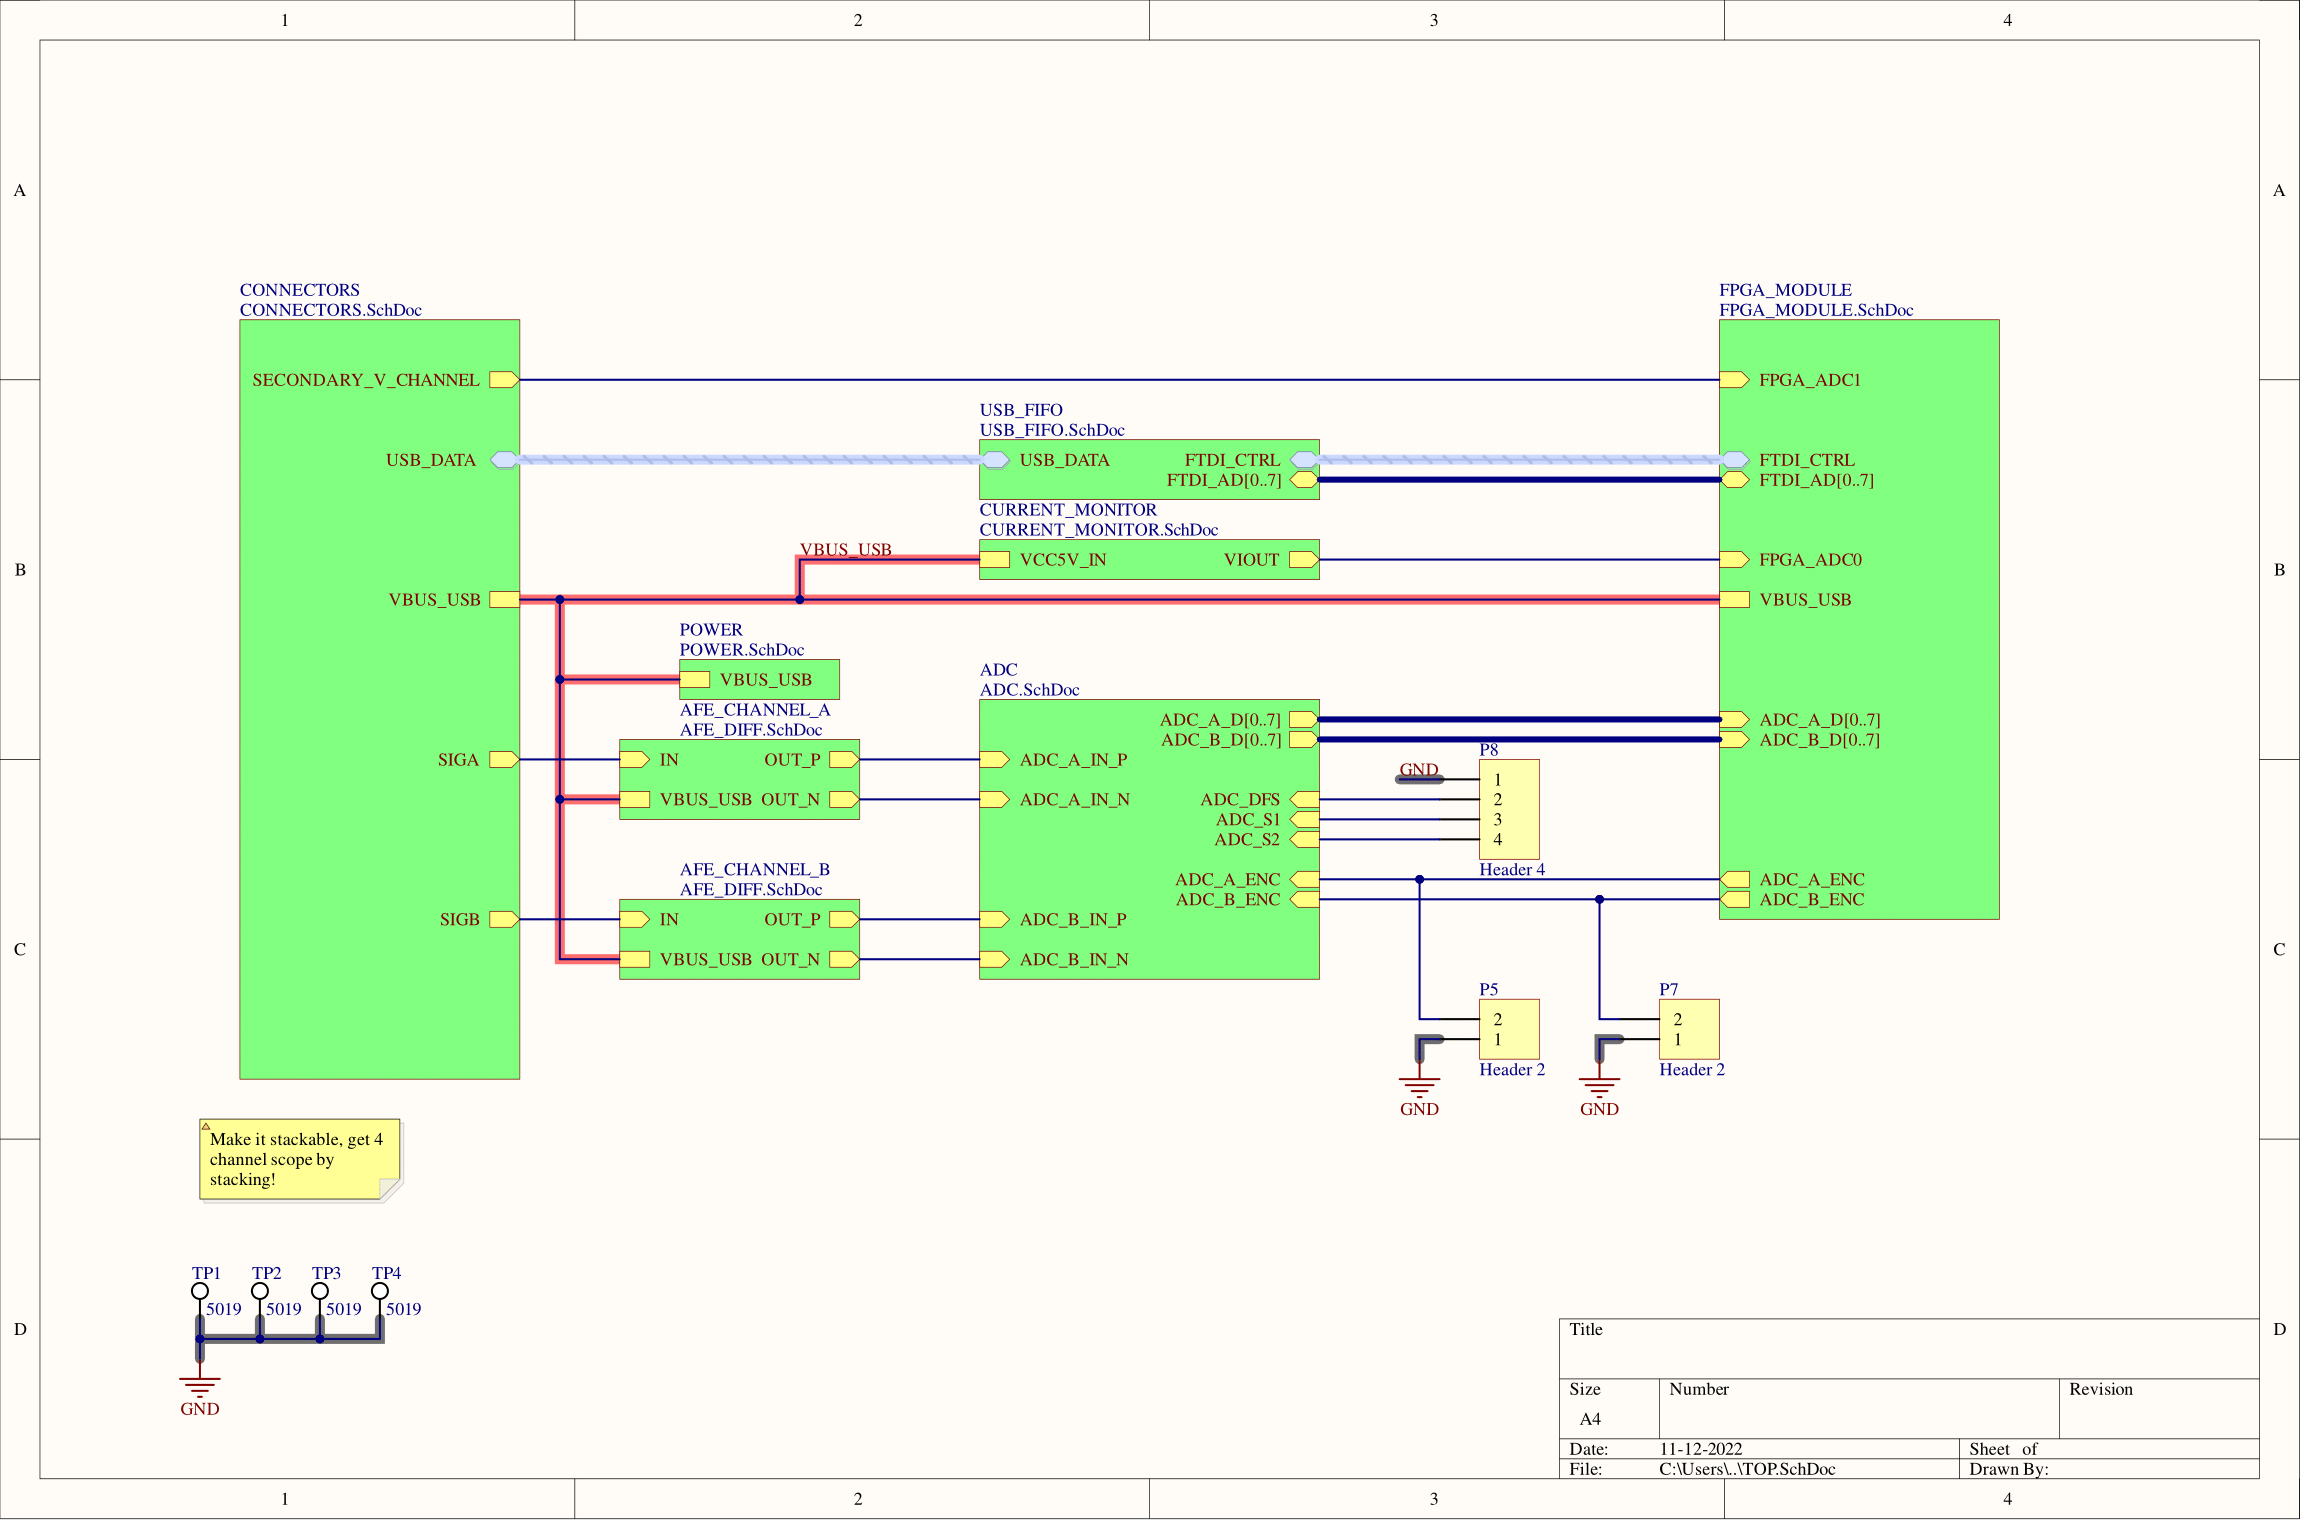
\includegraphics[height=15cm]{schematics/schematic1-1.png}
        \end{landscape}
    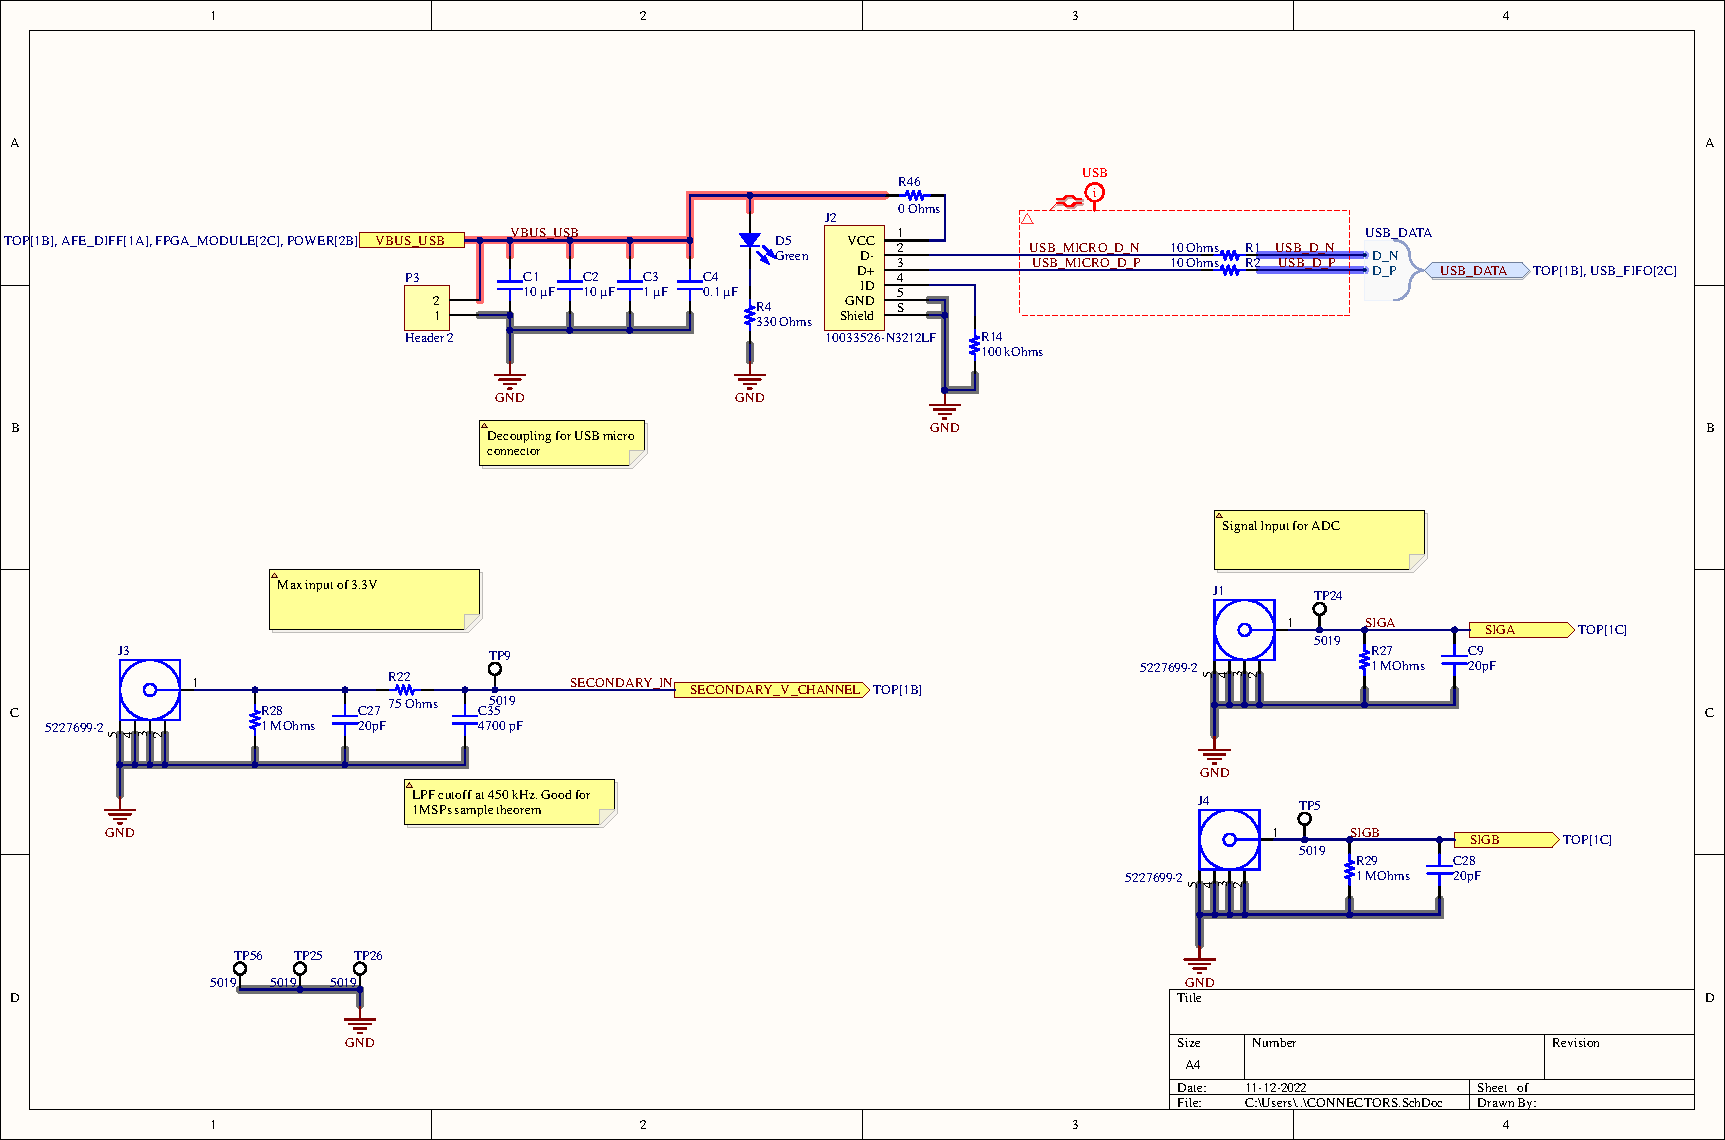
\includepdf[pages=-,landscape=true]{schematics/schematic2-8.pdf}

        \begin{landscape}
        \section{PCB Layout}
        \label{appendix:layout}
    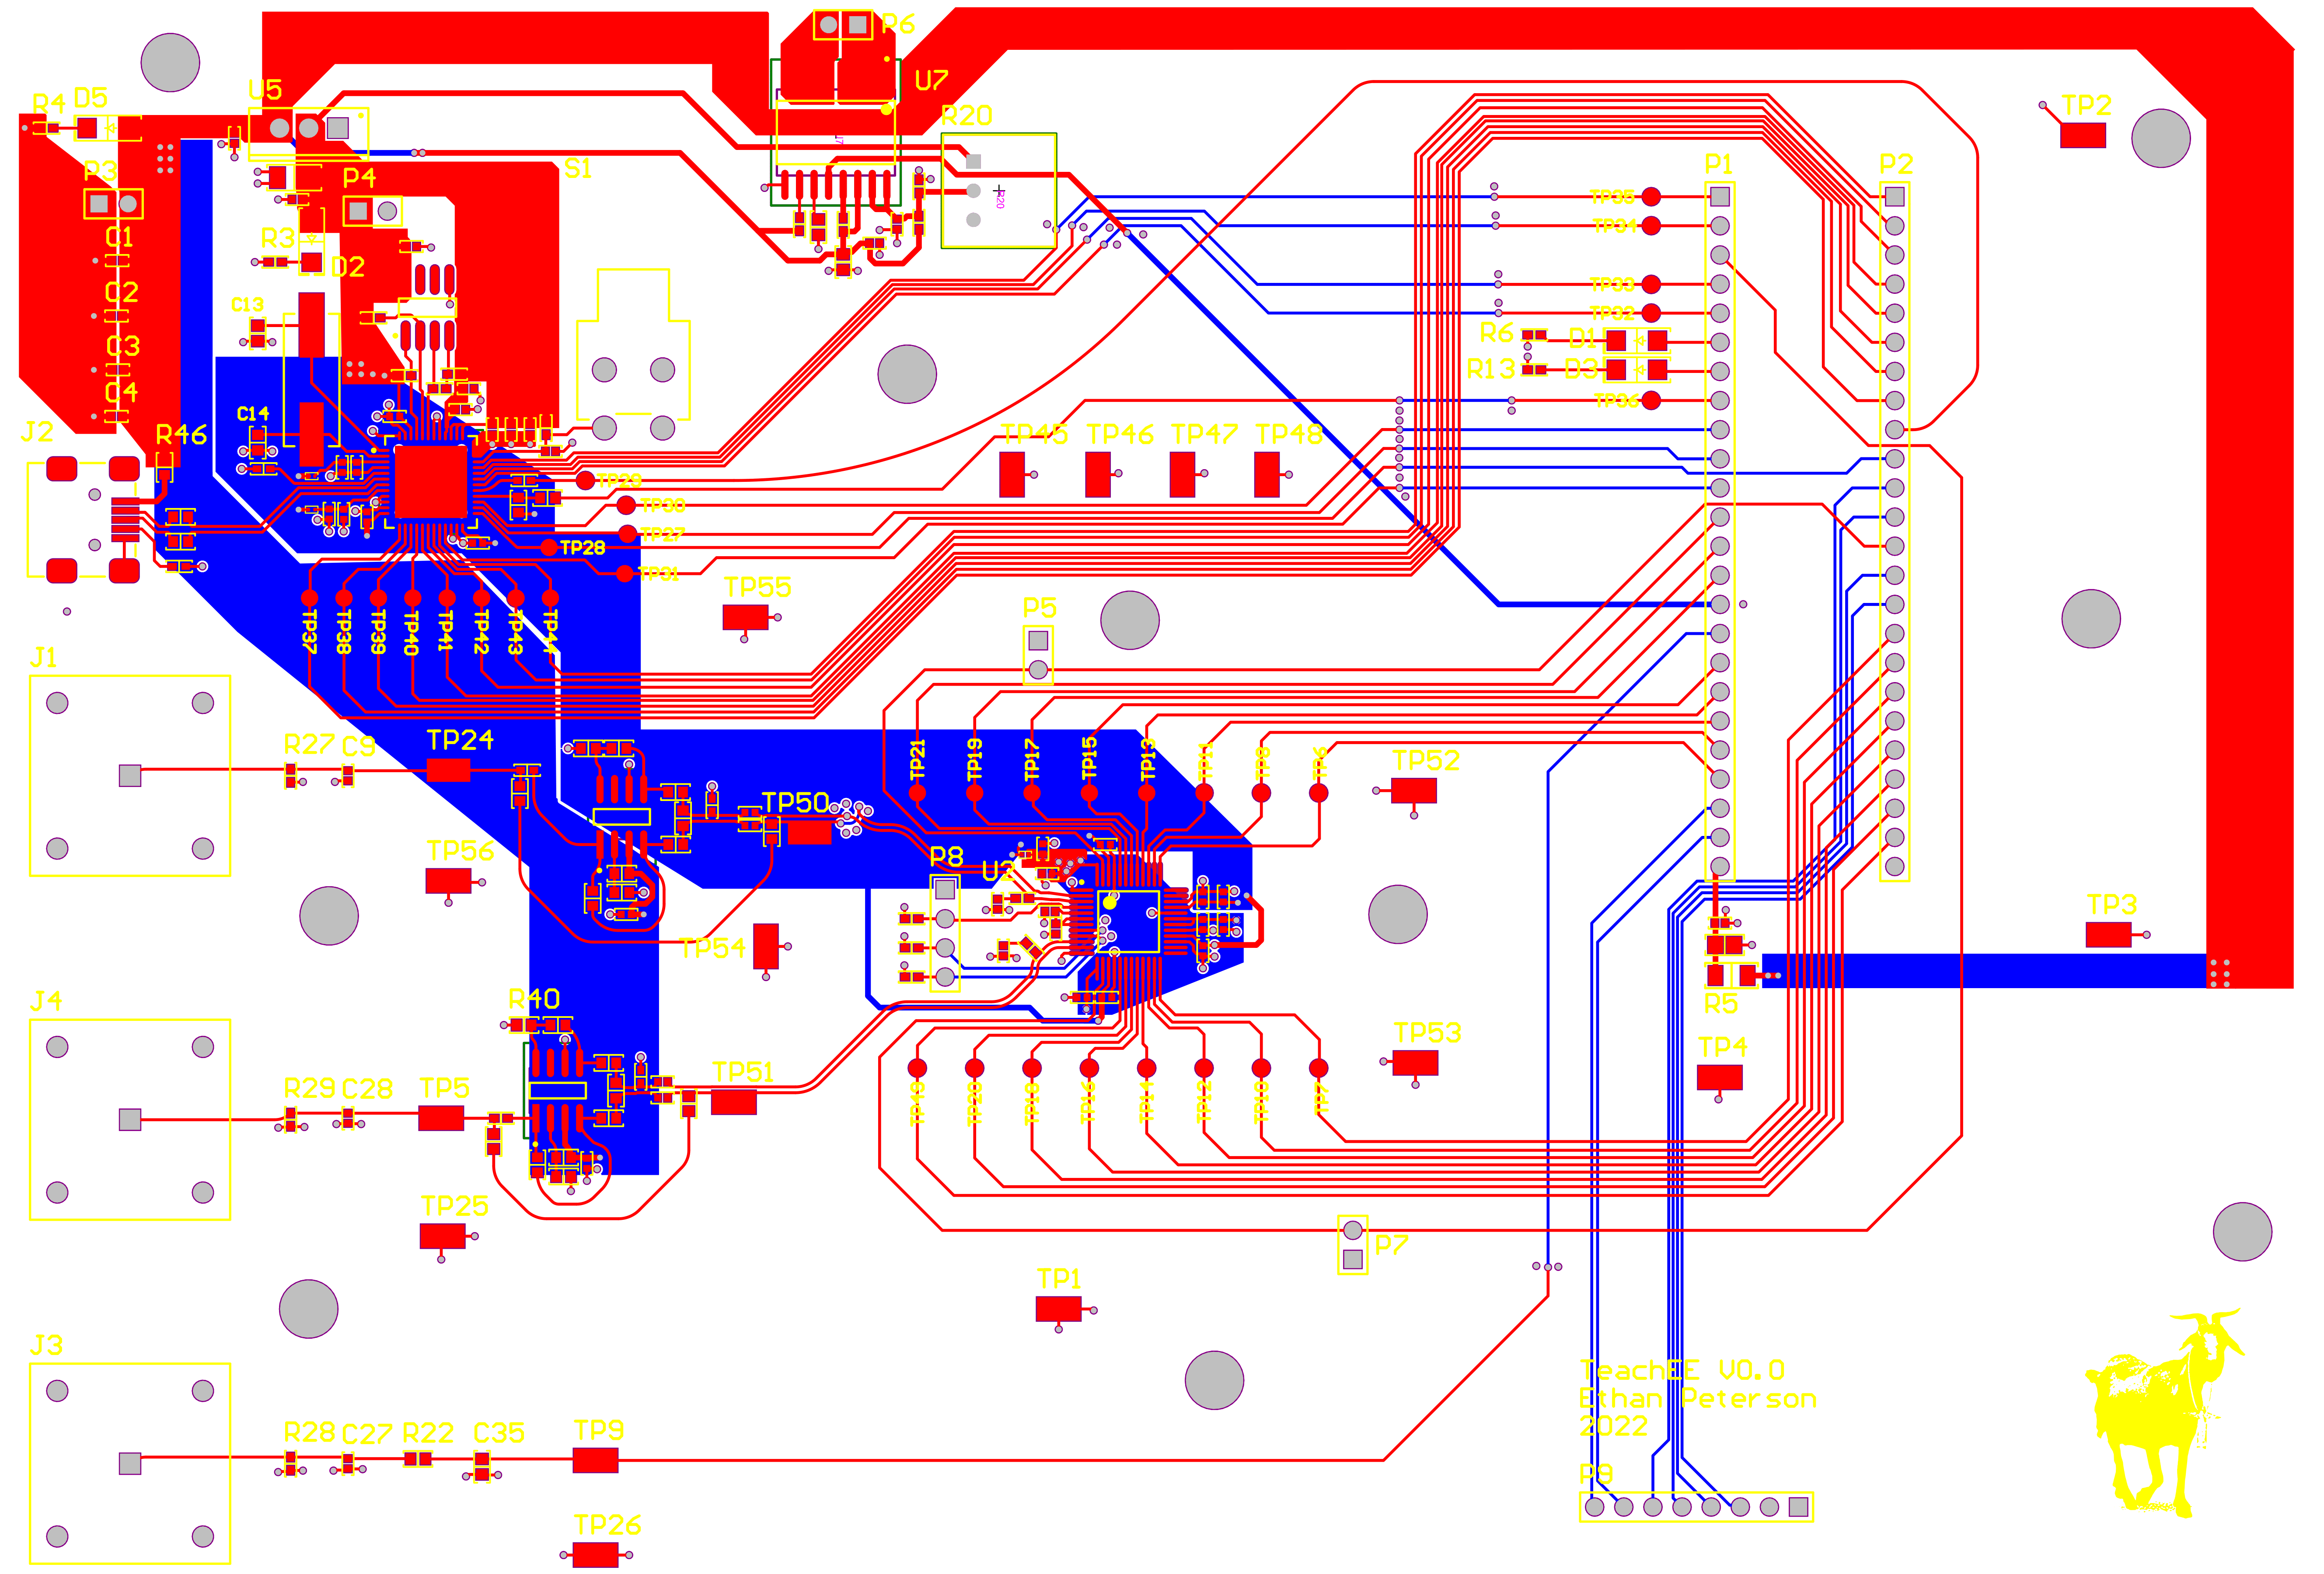
\includegraphics[height=15cm]{schematics/Layout.png}
        \end{landscape}

        \section{PCB Bill of Materials}
        \label{appendix:bom}
    \begin{table}[H]
    \begin{tabular}{p{1.7in}|p{0.3in}|p{0.8in}|p{0.7in}|p{0.7in}|p{1in}}
        \textbf{Designator} & \textbf{QTY} & \textbf{Description} & \textbf{Comment} & \textbf{Footprint} & \textbf{Part Number} \\ \hline 
        C1, C2, C37, C48 & 4 & CAP CER 10UF 10V X5R 0402 & 10 µF & CAP 0402\_1005 & CL05A106MP8NUB8 \\ \hline
        C3 & 1 & CAP CER 1UF 10V X7S 0402 & 1 µF & CAP 0402\_1005 & GRM155C71A105KE11D \\ \hline
        C4, C11, C16, C17, C18, C19, C20, C21, C22, C24, C26, C29, C30, C38, C39, C40, C41, C42, C43, C44, C45, C46, C47, C50\_AFE\_CHANNEL\_A, C50\_AFE\_CHANNEL\_B, C52\_AFE\_CHANNEL\_A, C52\_AFE\_CHANNEL\_B, C53\_AFE\_CHANNEL\_A, C53\_AFE\_CHANNEL\_B & 29 & CAP CER 0.1UF 50V X5R 0402 & 0.1 µF & CAP 0402\_1005 & CGA2B3X5R1H104M050BB \\ \hline
        C5, C12, C32, C34 & 4 & CAP CER 0.1UF 10V X7R 0402 & 0.1µF & CAP 0402\_1005 & 0402ZC104KAT2A \\ \hline
        C6 & 1 & CAP CER 10UF 16V X5R 1206 & 10 µF & CAP 1206\_3216 - 0.8MM & EMK316BJ106MD-T \\ \hline
        C7 & 1 & CAP CER 10UF 35V X6S 0805 & 10 µF & CAP 0805\_2012 & GRM21BC8YA106KE11L \\ \hline
        C8, C15, C23, C25 & 4 & CAP CER 4.7UF 16V X5R 0402 & 4.7 µF & CAP 0402\_1005 & CL05A475MO5NUNC \\ \hline
        C9, C27, C28 & 3 & CAP CER 20PF 25V NP0 0402 & 20pF & CAP 0402\_1005 & 04023U200JAT2A \\ \hline
    \end{tabular}
    \end{table}

    \newpage

    \begin{table}[H]
    \begin{tabular}{p{1.7in}|p{0.3in}|p{0.8in}|p{0.7in}|p{0.7in}|p{1in}}
        \textbf{Designator} & \textbf{QTY} & \textbf{Description} & \textbf{Comment} & \textbf{Footprint} & \textbf{Part Number} \\ \hline 
        C10 & 1 & CAP MLCC 0.01UF 100V X7R 0402 & 10000 pF & CAP 0402\_1005 & HMK105B7103KVHFE \\ \hline
        C13, C14 & 2 & CAP CER 36PF 100V NP0 0603 & 36pF & CAP 0603\_1608 & 06031A360JAT2A \\ \hline
        C31 & 1 & CAP CER 1UF 16V X7R 0603 & 1 µF & CAP 0603\_1608 & C0603C105K4RACAUTO \\ \hline
        C33, C35 & 2 & CAP CER 0603 4.7NF 16V X7R 10\% & 4700 pF & CAP 0603\_1608 & C0603C472K4RECAUTO \\ \hline
        C51\_AFE\_CHANNEL\_A, C51\_AFE\_CHANNEL\_B & 2 & CAP CER 15PF 25V C0G/NP0 0603 & 15 pF & CAP 0603\_1608 & C0603C150J3GACAUTO \\ \hline
        D1, D3 & 2 & LED SMD & Blue & LED 1206\_3216 BLUE & APTL3216QBC/D-01 \\ \hline
        D2, D5 & 2 & LED SMD & Green & LED 1206\_3216 GREEN & APTL3216ZGCK-01 \\ \hline
        FB1, FB2, FB3 & 3 & FERRITE BEAD 33 OHM 0201 1LN & 33 Ohms @ 100 MHz & FER 0201\_0603 & MMZ0603F330CT000 \\ \hline
        J1, J3, J4 & 3 & Jack BNC Connector, 1 Position, Height 16.26 mm, Tail Length 6.35 mm, -55 to 85 degC, RoHS, Tube & 5227699-2 & & 5227699-2 \\ \hline
        J2 & 1 & CONN RCPT MINI USB B 5POS SMD RA & & & 10033526-N3212LF \\ \hline
    \end{tabular}
    \end{table}
    \newpage
    \begin{table}[H]
        \begin{tabular}{p{1.7in}|p{0.3in}|p{0.8in}|p{0.7in}|p{0.7in}|p{1in}}
        \textbf{Designator} & \textbf{QTY} & \textbf{Description} & \textbf{Comment} & \textbf{Footprint} & \textbf{Part Number} \\ \hline 
        R1, R2 & 2 & RES SMD 10 OHM 0.1\% 1/10W 0603 & 10 Ohms & RES 0603\_1608 & CRT0603-BY-10R0ELF \\ \hline
        R3, R6, R13 & 3 & RES 220 OHM 1\% 1/8W 0402 & 220 Ohms & RES 0402\_1005 & CRGP0402F220R \\ \hline
        R4 & 1 & RES SMD 330 OHM 5\% 1/16W 0402 & 330 Ohms & RES 0402\_1005 & AC0402JR-07330RL \\ \hline
        R5 & 1 & 1206 40 AMP JUMPER & 0 Ohms & RES 1206\_3216 & JR1206X40E \\ \hline
        R7 & 1 & RES SMD 12K OHM 0.1\% 1/16W 0402 & 12 kOhms & RES 0402\_1005 & CPF0402B12KE1 \\ \hline
        R8, R9, R10, R11, R17, R18, R19, R21, R32, R33, R34 & 11 & RES 10K OHM 0.1\% 1/10W 0402 & 10 kOhms & RES 0402\_1005 & RP73PF1E10KBTD \\ \hline
        R12 & 1 & RES 1.8K OHM 1\% 1/16W 0402 & 1.8 kOhms & RES 0402\_1005 & RC0402FR-071K8L \\ \hline
        R14 & 1 & RES SMD 100K OHM 0.1\% 1/16W 0402 & 100 kOhms & RES 0402\_1005 & CPF0402B100KE \\ \hline
        R15, R46 & 2 & RES SMD 0 OHM JUMPER 1/2W 0603 & 0 Ohms & RES 0603\_1608 & 5110 \\ \hline
        R22 & 1 & RES SMD 75 OHM 1\% 1/10W 0603 & 75 Ohms & RES 0603\_1608 & AC0603FR-0775RL \\ \hline
        R26 & 1 & RES 24 OHM 1\% 1/16W 0402 & 24 Ohms & RES 0402\_1005 & RC0402FR-0724RL \\ \hline
        \end{tabular}
    \end{table}
    \newpage
    \begin{table}[H]
        \begin{tabular}{p{1.7in}|p{0.3in}|p{0.8in}|p{0.7in}|p{0.7in}|p{1in}}
        \textbf{Designator} & \textbf{QTY} & \textbf{Description} & \textbf{Comment} & \textbf{Footprint} & \textbf{Part Number} \\ \hline 
        R27, R28, R29 & 3 & RES 1M OHM 1\% 1/16W 0402 & 1 MOhms & RES 0402\_1005 & RMCF0402FT1M00 \\ \hline
        R36\_AFE\_CHANNEL\_A, R36\_AFE\_CHANNEL\_B & 2 & RES SMD 523 OHM 0.1\% 1/16W 0402 & 523 Ohms & RES 0402\_1005 & ERA-2ARB5230X \\ \hline
        R37\_AFE\_CHANNEL\_A, R37\_AFE\_CHANNEL\_B, R40\_AFE\_CHANNEL\_A, R40\_AFE\_CHANNEL\_B, R41\_AFE\_CHANNEL\_A, R41\_AFE\_CHANNEL\_B & 6 & RES SMD 500 OHM 0.05\% 1/10W 0603 & 500 Ohms & RES 0603\_1608 & TNPU0603500RAZEN00 \\ \hline
        R39\_AFE\_CHANNEL\_A, R39\_AFE\_CHANNEL\_B, R43\_AFE\_CHANNEL\_A, R43\_AFE\_CHANNEL\_B & 4 & RES 50 OHM 5\% 1/8W 0603 & 50 Ohms & RES 0603\_1608 & CH0603-50RJNTA \\ \hline
        R42\_AFE\_CHANNEL\_A, R42\_AFE\_CHANNEL\_B & 2 & RES SMD 4.02K OHM 1\% 1/10W 0603 & 4.02 kOhms & RES 0603\_1608 & AC0603FR-074K02L \\ \hline
        R44\_AFE\_CHANNEL\_A, R44\_AFE\_CHANNEL\_B & 2 & RES SMD 1K OHM 1\% 1/10W 0603 & 1 kOhms & RES 0603\_1608 & AA0603FR-071KL \\ \hline
        R45\_AFE\_CHANNEL\_A, R45\_AFE\_CHANNEL\_B & 2 & RES 25 OHM 0.1\% 1/20W 0402 & 25 Ohms & RES 0402\_1005 & FC0402E25R0BST0 \\ \hline
        S1 & 1 & SWITCH PUSH SPST-NO 0.4VA 28V & &  & AB11AH-HA \\ \hline
        TP1, TP2, TP3, TP4, TP5, TP9, TP24, TP25, TP26, TP45, TP46, TP47, TP48, TP50, TP51, TP52, TP53, TP54, TP55, TP56 & 20 & Test Point, 1 Position SMD, RoHS, Tape and Reel & 5019 & KSTN5019 & 5019 \\ \hline
        U1 & 1 & IC HS USB TO UART/FIFO 48QFN & FT232 & QFN-48 & FT232HQ-REEL \\ \hline
        \end{tabular}
    \end{table}
    \newpage
    \begin{table}[H]
        \begin{tabular}{p{1.7in}|p{0.3in}|p{0.8in}|p{0.7in}|p{0.7in}|p{1in}}
        \textbf{Designator} & \textbf{QTY} & \textbf{Description} & \textbf{Comment} & \textbf{Footprint} & \textbf{Part Number} \\ \hline 
        U2 & 1 & Dual 8-Bit AD Converter with Parallel Interface, 40MSPS, -40 to +85 degC, ST-48, Pb-Free, Tray &  & ST-48M & AD9288BSTZ-40 \\ \hline
        U3\_AFE\_CHANNEL\_A, U3\_AFE\_CHANNEL\_B & 2 & IC ADC DRIVER 8SOIC & AD8138 & R-8-IPC\_A & AD8138ARZ-R7 \\ \hline
        U5 & 1 & Fixed Low Drop Positive Voltage Regulator, 3.3V, 3-Pin TO-220 & LD1117 & TO220 & LD1117V33C \\ \hline
        U6 & 1 & 2K, 128x16-bit, 2.5V Microwire Serial EEPROM, 8-Pin SOIC 150mil, Commercial Temperature, Tape and Reel & 93LC56 & SOIC8 & 93LC56BT/SN \\ \hline
        U7 & 1 & CURRENT SENSOR & ACS720 &  & ACS720KLATR-15AB-T \\ \hline
        Y1 & 1 & CRYSTAL 12.0000MHZ 20PF SMD & 12 MHz & ABLS & ABLS-12.000MHZ-20-B-3-H-T \\ \hline
        \end{tabular}
    \end{table}

    % TODO: needs smaller font size or line wrapping
    \section{TeachEE SystemVerilog RTL Code} \label{appendix:rtl-code}
    This appendix contains all the SystemVerilog RTL files in the TeachEE
    project. Each subsection corresponds to the files in a particular folder of
    the GitHub repository.

    \subsubsection{TeachEE Main Project Top Level Module}
    \inputminted[linenos,breaklines]{systemverilog}{../../rtl/teachee/teachee.sv}

    \subsection{AXIS} \label{appendix:axis}
    \subsubsection{axis\_adapter\_wrapper.sv}
    \inputminted[linenos,breaklines]{systemverilog}{../../rtl/axis/axis_adapter_wrapper.sv}
    \subsubsection{axis\_async\_fifo\_wrapper.sv}
    \inputminted[linenos,breaklines]{systemverilog}{../../rtl/axis/axis_async_fifo_wrapper.sv}
    \subsubsection{axis\_interface.sv} \label{appendix:axis-interface}
    \inputminted[linenos,breaklines]{systemverilog}{../../rtl/axis/axis_interface.sv}

    \subsection{COBS}
    \subsubsection{cobs\_axis\_adapter\_wrapper.sv}
    \inputminted[linenos,breaklines]{systemverilog}{../../rtl/cobs/cobs_axis_adapter_wrapper.sv}
    \subsubsection{cobs\_encode\_wrapper.sv}
    \inputminted[linenos,breaklines]{systemverilog}{../../rtl/cobs/cobs_encode_wrapper.sv}

    \subsection{FT232H}
    \subsubsection{ft232h.sv}
    \inputminted[linenos,breaklines]{systemverilog}{../../rtl/ft232h/ft232h.sv}
    \subsubsection{ft232h\_bfm.sv}
    \inputminted[linenos,breaklines]{systemverilog}{../../rtl/ft232h/ft232h_bfm.sv}
    \subsubsection{ft232h\_package.sv}
    \inputminted[linenos,breaklines]{systemverilog}{../../rtl/ft232h/ft232h_package.sv}

    \subsection{HSADC}
    \subsubsection{hsadc\_axis\_wrapper.sv}
    \inputminted[linenos,breaklines]{systemverilog}{../../rtl/hsadc/hsadc_axis_wrapper.sv}
    \subsubsection{hsadc\_bfm.sv}
    \inputminted[linenos,breaklines]{systemverilog}{../../rtl/hsadc/hsadc_bfm.sv}
    \subsubsection{hsadc\_interface.sv}
    \inputminted[linenos,breaklines]{systemverilog}{../../rtl/hsadc/hsadc_interface.sv}

    \subsection{Xilinx XADC} \label{xadc-bfm}
    \subsubsection{xadc\_bfm.sv}
    \inputminted[linenos,breaklines]{systemverilog}{../../rtl/xadc/xadc_bfm.sv}
    \subsubsection{xadc\_drp\_axis\_adapter.sv}
    \inputminted[linenos,breaklines]{systemverilog}{../../rtl/xadc/xadc_drp_axis_adapter.sv}
    \subsubsection{xadc\_drp\_axis\_single\_stream.sv}
    \inputminted[linenos,breaklines]{systemverilog}{../../rtl/xadc/xadc_drp_axis_single_stream.sv}
    \subsubsection{xadc\_drp\_package.sv}
    \inputminted[linenos,breaklines]{systemverilog}{../../rtl/xadc/xadc_drp_package.sv}
    \subsubsection{xadc\_packetizer.sv}
    \inputminted[linenos,breaklines]{systemverilog}{../../rtl/xadc/xadc_packetizer.sv}

    \subsection{Legacy Non-VUnit Testbenches} \label{appendix:rtl-leg-tb}
    \subsubsection{ft232h\_bfm\_tb.sv}
    \inputminted[linenos,breaklines]{systemverilog}{../../rtl/testbenches/legacy/ft232h_bfm_tb.sv}
    \subsubsection{ft232h\_tb.sv}
    \inputminted[linenos,breaklines]{systemverilog}{../../rtl/testbenches/legacy/ft232h_tb.sv}
    \subsubsection{xadc\_bfm\_tb.sv}
    \inputminted[linenos,breaklines]{systemverilog}{../../rtl/testbenches/legacy/xadc_bfm_tb.sv}
    \subsubsection{xadc\_drp\_axis\_adapter\_tb.sv}
    \inputminted[linenos,breaklines]{systemverilog}{../../rtl/testbenches/legacy/xadc_drp_axis_adapter_tb.sv}

    \subsection{VUnit Testbenches} \label{appendix:rtl-vunit-tb}
    \subsubsection{axis\_adapter\_wrapper\_tb.sv}
    \inputminted[linenos,breaklines]{systemverilog}{../../rtl/testbenches/axis_adapter_wrapper_tb.sv}
    \subsubsection{cobs\_axis\_adapter\_wrapper\_tb.sv}
    \inputminted[linenos,breaklines]{systemverilog}{../../rtl/testbenches/cobs_axis_adapter_wrapper_tb.sv}
    \subsubsection{cobs\_encode\_wrapper\_tb.sv}
    \inputminted[linenos,breaklines]{systemverilog}{../../rtl/testbenches/cobs_encode_wrapper_tb.sv}
    \subsubsection{hsadc\_axis\_wrapper\_tb.sv}
    \inputminted[linenos,breaklines]{systemverilog}{../../rtl/testbenches/hsadc_axis_wrapper_tb.sv}
    \subsubsection{xadc\_packetizer\_tb.sv}
    \inputminted[linenos,breaklines]{systemverilog}{../../rtl/testbenches/xadc_packetizer_tb.sv}

    \subsection{Example Projects}
    \subsubsection{blink}
    \inputminted[linenos,breaklines]{systemverilog}{../../rtl/examples/blink/blink.sv}
    \subsubsection{ftdi\_sync}
    \inputminted[linenos,breaklines]{systemverilog}{../../rtl/examples/ftdi_sync/ftdi_sync.sv}
    \subsubsection{pll\_blink}
    \inputminted[linenos,breaklines]{systemverilog}{../../rtl/examples/pll_blink/pll_blink.sv}
    \subsubsection{xadc\_axis}
    \inputminted[linenos,breaklines]{systemverilog}{../../rtl/examples/xadc_axis/xadc_axis.sv}

    \section{FPGA GitHub Actions Script} \label{appendix:github-action-script}
    \inputminted[linenos,breaklines]{yaml}{../../.github/workflows/rtl.yml}

    \section{Python VUnit Testbenches} \label{appendix:python-vunit-tb}
    \subsection{axis\_adapter\_wrapper\_tb.py}
    \inputminted[linenos,breaklines]{python}{../../rtl/python/axis_adapter_wrapper_tb.py}
    \subsection{cobs\_axis\_adapter\_wrapper\_tb.py}
    \inputminted[linenos,breaklines]{python}{../../rtl/python/cobs_axis_adapter_wrapper_tb.py}
    \subsection{cobs\_encode\_wrapper\_tb.py}
    \inputminted[linenos,breaklines]{python}{../../rtl/python/cobs_encode_wrapper_tb.py}
    \subsection{hsadc\_axis\_wrapper\_tb.py}
    \inputminted[linenos,breaklines]{python}{../../rtl/python/hsadc_axis_wrapper_tb.py}
    \subsection{xadc\_packetizer\_tb.py}
    \inputminted[linenos,breaklines]{python}{../../rtl/python/xadc_packetizer_tb.py}

    \section{Python Packet Integrity Test Script} \label{appendix:python-reader}
    \inputminted[linenos,breaklines]{python}{../../rtl/teachee/reader.py}

    \section{TeachEE Rust Code} \label{appendix:software}

    \subsection{main.rs}
    \inputminted[linenos,breaklines]{rust}{../../software/teachee-desktop/src/main.rs}

    \subsection{/sample\_source} \label{appendix:software-usb_manager}

    \subsubsection{mod.rs} \label{appendix:software-mod}
    \inputminted[linenos,breaklines]{rust}{../../software/teachee-desktop/src/sample_source/mod.rs}

    \subsubsection{ft.rs} \label{appendix:software-ft}
    \inputminted[linenos,breaklines]{rust}{../../software/teachee-desktop/src/sample_source/ft.rs}

    \subsubsection{sine.rs} \label{appendix:software-sine}
    \inputminted[linenos,breaklines]{rust}{../../software/teachee-desktop/src/sample_source/sine.rs}

    \subsection{controller.rs} \label{appendix:software-controller}
    \inputminted[linenos,breaklines]{rust}{../../software/teachee-desktop/src/controller.rs}

    \subsection{app.rs} \label{appendix:software-app}
    \inputminted[linenos,breaklines]{rust}{../../software/teachee-desktop/src/app.rs}

    \subsection{xtask: main.rs} \label{appendix:software-script}
    \inputminted[linenos,breaklines]{rust}{../../software/teachee-desktop/xtask/src/main.rs}

    \end{appendices}
\end{document}
